\documentclass[defaultstyle,11pt]{thesis}

%%%%%%%%%%%%%%%%%%%%%%%%%%%%%%%%%%%%%%%%%%%%%%%%%%%%%%%%%%%%%%%%
%%%%%%%%%%%  see documentation for information about  %%%%%%%%%%
%%%%%%%%%%%  the options (11pt, defaultstyle, etc.)   %%%%%%%%%%
%%%%%%%  http://www.colorado.edu/its/docs/latex/thesis/  %%%%%%%
%%%%%%%%%%%%%%%%%%%%%%%%%%%%%%%%%%%%%%%%%%%%%%%%%%%%%%%%%%%%%%%%
%		\documentclass[typewriterstyle]{thesis}
% 		\documentclass[modernstyle]{thesis}
% 		\documentclass[modernstyle,11pt]{thesis}
%	 	\documentclass[modernstyle,12pt]{thesis}

%%%%%%%%%%%%%%%%%%%%%%%%%%%%%%%%%%%%%%%%%%%%%%%%%%%%%%%%%%%%%%%%
%%%%%%%%%%%    load any packages which are needed    %%%%%%%%%%%
%%%%%%%%%%%%%%%%%%%%%%%%%%%%%%%%%%%%%%%%%%%%%%%%%%%%%%%%%%%%%%%%
\usepackage{latexsym}		% to get LASY symbols
\usepackage{graphicx}		% to insert PostScript figures
\usepackage{rotating}		% for sideways tables/figures
\usepackage{verbatim}
\usepackage{moreverb}
\usepackage{epsfig}
\usepackage{subfigure}
\usepackage{times}
\usepackage{amssymb}
\usepackage{amsmath}
\usepackage{algorithm2e}
\usepackage{amsfonts}
\usepackage{epstopdf}
\usepackage{multirow}
\usepackage{url}
\usepackage{verbatim}
\usepackage{listings}
\usepackage{footmisc}
\usepackage{longtable}
\usepackage{threeparttable}
\usepackage{subfigure}
\usepackage[sort]{cite}
%%%%%%%%%%%%%%%%%%%%%%%%%%%%%%%%%%%%%%%%%%%%%%%%%%%%%%%%%%%%%%%%
%%%%%%%%%%%%       all the preamble material:       %%%%%%%%%%%%
%%%%%%%%%%%%%%%%%%%%%%%%%%%%%%%%%%%%%%%%%%%%%%%%%%%%%%%%%%%%%%%%
\title{Enabling Dynamic Voltage and Frequency Scaling in Multicore Architectures}

\author{Amithash}{Prasad}

\otherdegrees{B.S., Visveswaraya Technical University, 2005 }

\degree{Master of Science}		%  #1 {long descr.}
	{M.S., Computer Engineering}		%  #2 {short descr.}

\dept{Department of}			%  #1 {designation}
	{Electrical and Computer Engineering}		%  #2 {name}

\advisor{}				%  #1 {title}
	{Prof. Manish Vachharajani (chair)}			%  #2 {name}

\reader{Prof. Dan Connors}		%  2nd person to sign thesis
\readerThree{Prof. Dirk Grunwald}		%  3nd person to sign thesis

\abstract{  \OnePageChapter	% one page only ??

Traditionally, patterns and repetition in program behavior are
exploited in multiple ways to increase performance in computer
systems.  Cache memory and branch prediction are examples of hardware
technologies that leverage short-term knowledge of program behavior to
enhance performance.  On a different scale, profile-guided compiler
transformations use profile information to customize optimization
decisions to program behavior. However, as the microprocessor industry
shifts to multi-core designs, continued performance gains can only be
achieved by systems that track and adapt to interactions of multiple
concurrent programs.  Multiple cores per system do not universally
improve performance since shared resources and operating conditions
cause interference.  To optimally manage and design multi-core systems
so that they may achieve continued performance gains, new methods of
representing and exploiting program execution behavior are required.

This thesis presents a new representation, the Cardinal Execution Map
(CEM), which describes phase-based program behavior in a compact form.
The representation aids computer system design, helps analyze resource
contention in multi-core environments and directs run-time systems to
better utilize hardware.  The Cardinal Execution Map can be
constructed off-line (statically) and at run time (dynamically) to
enhance the study of microarchitecture, program behaviors, and
multi-core systems.  Presented in the thesis are the execution
modeling framework, a set of analyzes for execution prediction and
program behavior identification, and a multi-context program interaction
modeling system.


}


\dedication[Dedication]{	% NEVER use \OnePageChapter here.
This thesis is dedicated to my fiance Sushma

}

\acknowledgements{	\OnePageChapter	% *MUST* BE ONLY ONE PAGE!
First, I would like to thank my advisers Dan Connors and Manish Vachharajani 
for their advice, tutoring, and incredible patience. I am grateful for the courses they 
taught which got me interested in computer engineering and lured me away
from control systems which was my initial idea of a master's degree.

Second, I'd like to thank Professor Dirk Grunwald for his motivation and 
suggestions every time I stumbled into his office without an appointment
which shows the level of his patience and the willingness to help.  

Third, I'd like to thank Tipp Moseley a fellow graduate student for helping me
out during my initial introduction into kernel hacking, and answering 
my questions whenever I felt that I was somehow within the grasp of a black hole. 
This does not exclude the very helpful and friendly Linux kernel community 
who helped a novice transition into a real kernel hacker. This would not end 
without thanking Linus Torvalds for creating the Linux kernel in the first place.

Forth, I would like to thank my fiance Sushma for listening to me whine during 
the initial part of this thesis when whatever I touched seemed to crash; For 
listening to me gloat in pride when things worked for a change, and finally
for proof reading my thesis when I realized that I have forgotten the entire
English language.

Finally, I'd like to thank my parents for motivating me all along, my friends 
for helping in proof reading my thesis document and answering any questions I had
along the way. 
}

\ToCisShort	% a 1-page Table of Contents ??

\LoFisShort	% a 1-page List of Figures ??
%	\emptyLoF	% no List of Figures at all ??

\LoTisShort	% a 1-page List of Tables ??
%	\emptyLoT	% no List of Tables at all ??


\begin{document}
%%%%%%%%%%%%%%%%%%%%%%%%%%%%%%%%%%%%%%%%%%%%%%%%%%%%%%%%%%%%%%%%%
%%%%%%%%%%%%%%%       BEGIN DOCUMENT...         %%%%%%%%%%%%%%%%%
%%%%%%%%%%%%%%%%%%%%%%%%%%%%%%%%%%%%%%%%%%%%%%%%%%%%%%%%%%%%%%%%%

%%%%%%%%%%%%%%%%%%%%%%%%%%%%%%%%%%%%%%%%%%%%%%%%%%%%%%%%%%%%%%%%%%%%%%%%%%%%%%%
\chapter{Introduction}~\label{chap:intro}
%%%%%%%%%%%%%%%%%%%%%%%%%%%%%%%%%%%%%%%%%%%%%%%%%%%%%%%%%%%%%%%%%%%%%%%%%%%%%%%


% Opening overview
Several technology constraints are threatening to slow the rate of
growth in computer system performance. Specifically, current designers
are finding difficulties addressing strict processor power consumption
and cooling constraints.  Design modifications to address power
consumption generally limit processor performance and reduce peak
operating frequency, thus changing the trend of providing increased
system performance every new processor generation.  As such, modern
architectures have diverged from the clock speed race into the
multi-core era with multiple processing cores on a single die. While
the multi-core design strategy improves chip power density, there
remains a significant potential in improving run-time power
utilization by dynamically changing per-core clock frequency and
voltage.

% WHAT IS DVFS
Power consumption has been observed to be 
directly proportional to the clock speed (frequency) and the 
square of the operating voltage of the processor 
($Power \propto frequency \times Voltage^2$). In order to conserve energy, designers have explored methods to
manipulate these parameters at runtime.
Implementations of DVFS schemes divides the processor operation in islands called 
performance states or P-states with fixed operating voltage and clock speeds. 
Architectures supporting DVFS mechanisms provide 2-8 such islands or DVFS configurations thus transforming
decisions in linear space to that in discrete space. 

Literature provides various schemes of manipulating DVFS configurations of a processor and
can be subdivided into three broad categories: hardware, operating system and compiler/runtime systems. 
DVFS at the architecture level, implemented 
in hardware to monitor and predict execution patterns and allowing the power optimizer
to react to such events to manipulate the system's DVFS configuration. These methods are 
presented and studied in \cite{SystemLevel}, \cite{Phaseaware} and \cite{ImprovingFairness}.
In-hardware methods are immutable implementations in silicon which cannot be changed based on
design and policy variations and hence avoided by many chip manufacturers who in turn rely on software for policy 
implementation and changes. Next 
\cite{MultiOptimization}, \cite{LiveRuntime}, \cite{OperatingSystem} and \cite{schedulerHPC} elevate these design 
considerations from the hardware to the operating system level which expect some form
of runtime performance monitoring capabilities exported from the hardware in order to measure 
and predict execution phase patterns to assist such operating system based power management systems.
Finally, the last category is the management of power controlled by compiler and user space runtime systems
which expect such capabilities to be exported by the operating system as discussed in \cite{dynamic_compiler_f},
\cite{AnIntraTask}, \cite{compilerDirectedDVFS} and trace driven methods for power management as discussed
in \cite{adagio} and \cite{boundingEnergy}.
 

Majority of DVFS (Dynamic Voltage and Frequency Scaling) implementations at the operating system level are load based where
the system's DVFS configuration is varied based upon the usage patters of the hardware. Even though
effective in conserving power, this methodology is unaware of the workload currently executing on
the system. Load based decisions
are best left to technologies which decide whether the processing element 
is active or asleep (The state at which the power consumption is minimal) and is studied in
\cite{OperatingSystem} which predicts usage patterns of various devices on the system. 

% Statement of work overview
This work proposes techniques which tie the scheduler and the system power optimizer to
constrain the number of DVFS level changes both over time and
intensity with the goal of  energy savings without harming
performance. Limiting DVFS level transitions becomes important to limit the instabilities endured by the system due to rapid
DVFS transitions as explored by \cite{ImpactDVFS}.

% Contributions
This thesis makes the following contributions to this area of study:
\begin{enumerate}
\item Method of scheduling to adjust DVFS with
strict constraints on limiting the amount of performance lost compared
to full frequency mode. The system provides significant power savings of up to 40\% 
with a performance loss of up to 20\% with a median performance loss at around 10-15\%.
\item Method to schedule tasks based on their performance requirement on a multi processor
environment with varying asymmetric clock speeds in order to maximize power savings
while minimizing performance lost. 
\item Investigation of the impact of DVFS level changes per second on the ability to improve power savings
or performance impact.
\item Devised a multi-task scheduling model that accounts for joule-per-instruction work metric.
\end{enumerate}

% Chapter Organization

This thesis is organized as follows:
Chapter~\ref{chap:pds} introduces the performance directed scheduler.
Chapter~\ref{chap:delta} proposes a methodology to mutate voltage and 
frequency configuration of a system based on the workload demands. 
Chapter~\ref{chap:results} describes the experimental procedure
and results obtained. Chapter~\ref{chap:future} comments on the future
work in this area and finally chapter~\ref{chap:conclusion} concludes this
thesis.   


%%%%%%%%%%%%%%%%%%%%%%%%%%%%%%%%%%%%%%%%%%%%%%%%%%%%%%%%%%%%%%%%%%%%%%%%%%%%%%%
\chapter{Performance directed scheduling on asymmetric multi-processors}~\label{chap:pds}
%%%%%%%%%%%%%%%%%%%%%%%%%%%%%%%%%%%%%%%%%%%%%%%%%%%%%%%%%%%%%%%%%%%%%%%%%%%%%%%

Current implementations of schedulers in modern operating systems recognize the environment
as homogeneous in nature while technologies such as DVFS (Dynamic Voltage and Frequency Scaling) introduce an
inherent asymmetry in a multiprocessor system. 
Considerable direction in terms of asymmetric scheduling support has been addressed in \cite{AsymmetricScheduling}
and \cite{Multitasking} but on the downside, the work does not consider the requirements of tasks in terms of capability
and speed of the processing element which brings little advantage to the existing system.

In a multi-core environment, there are many facets for performance loss with the most 
common reasons being high IO and memory latencies which is further aggravated by cache sharing.
A novel statistical learning method to predict voltage and frequency requirements by tasks 
was proposed in \cite{AnIntraTask}, but the method required rigorous statistical learning making it 
time consuming and impossible to implement at the context of a scheduler. A
simpler method was proposed in \cite{LiveRuntime} and \cite{Phaseaware}, but comes at the cost
of possible rapid voltage and frequency transitions which may lead to instabilities in emergencies
(Even with a quad core system and a scheduling frequency of 1000Hz, there is a possibility
of $1000 \times 4 = 4000$ performance state transitions every second) as shown in \cite{ImpactDVFS}. 

%%%%%%%%%%%%%%%%%%%%%%%%%%%%%%%%%%%%%%%%%%%%%%%%%%%%%%%%%%%%%%%%%%%%%%%%%%%%%%%
\section{Performance behavior of SPEC workloads}~\label{sec:perf_behav}
%%%%%%%%%%%%%%%%%%%%%%%%%%%%%%%%%%%%%%%%%%%%%%%%%%%%%%%%%%%%%%%%%%%%%%%%%%%%%%%

In order to study the behavior of real applications on different voltage and frequency settings,
fourteen of the SPEC2006 \cite{spec:2006} benchmark suite were run with varied clock speed 
from 1100 MHz to 2200 MHz on an AMD Opteron Quad core processor and were plotted showing the 
percentage duration spent at an IPC (Instruction per Clock) higher than 1.0 and the 
speed-up in terms of execution time achieved from that when run with the lowest clock speed (1100 MHz). 
This is shown in Figure~\ref{fig:spec_classify}.
The X-axis of this graph is the percentage of time the benchmark spent running at an IPC level greater
than 1.0, the Y-axis is the clock speed at which the benchmark was run at, and finally the Z-axis 
is the Speed-up achieved. It can be observed that the return on investment (Higher clock speed)
is low for tasks with a low percentage of runtime at an IPC greater than 1.0. Artificial workloads
comprising of 4 benchmarks each were created (shown in Table~\ref{tab:spec_groups}) based on their IPC classification
and real-world usage on throughput based systems. Figure~\ref{fig:group_speedup} shows that the workload 
\textit{High} category shows the greatest improvement with frequency, achieving a nearly 2x improvement using the highest
frequency for each core in the 4-core system.  Otherwise, the other
categories of workloads appear to benefit from higher frequency, but
are bounded to 1.5x of the baseline execution time.
This motivates the construction of a performance directed scheduler aware of the IPC
level at which tasks are executing and described in further sections. 

\begin{figure}[h!]
  \begin{center}
    %\resizebox{\columnwidth}{!}{
    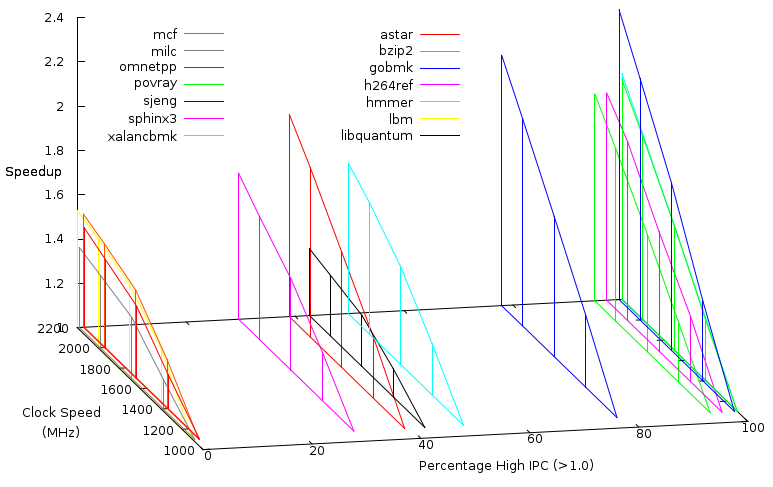
\includegraphics[height=3.5in]{figures/Speedup_Classify.png}%}
    \caption{IPC classification and speedup trends for the SPEC 2006 benchmarks}
    \label{fig:spec_classify}
  \end{center}
\end{figure}

\begin{figure}[h!]
  \begin{center}
    %\resizebox{\columnwidth}{!}{
    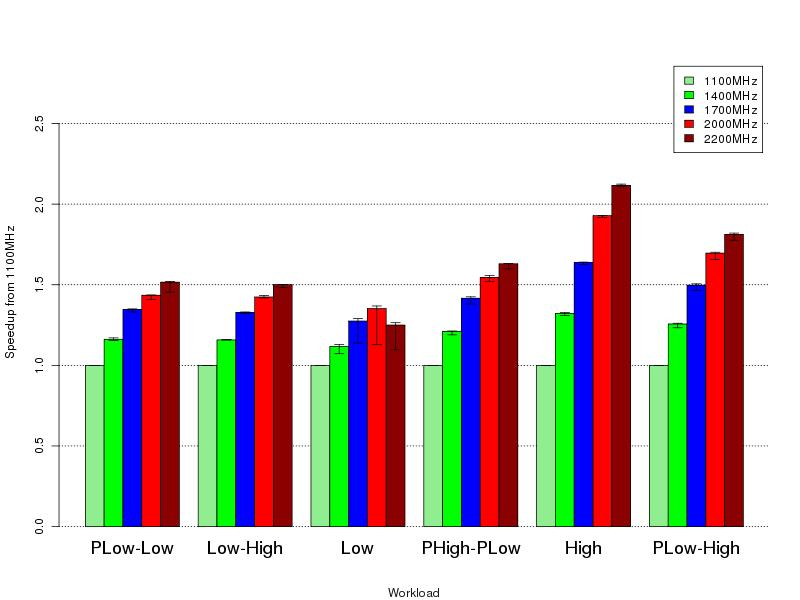
\includegraphics[height=3.5in]{figures/group_speedup.jpg}%}
    \caption{Speedup achieved by characterized workloads}
    \label{fig:group_speedup}
  \end{center}
\end{figure}

%%%%%%%%%%%%%%%%%%%%%%%%%%%%%%%%%%%%%%%%%%%%%%%%%%%%%%%%%%%%%%%%%%%%%%%%%%%%%%%
\section{Quantifying performance}~\label{sec:quant_perf}
%%%%%%%%%%%%%%%%%%%%%%%%%%%%%%%%%%%%%%%%%%%%%%%%%%%%%%%%%%%%%%%%%%%%%%%%%%%%%%%

An adaptive system needs a quantitative measure of performance. Section~\ref{sec:perf_behav} indicated
that IPC can be used as such a measure. In order to study the throughput and energy consumption behavior of
workloads, a hardware monitoring-based framework was constructed to
collect and correlate per-application IPC data. Figure~\ref{fig:ipc_speedup} 
was constructed displaying the speedup which was achieved in terms of throughput when compared to the same 
sample executed at the base clock speed of 1100 MHz. This provides an aid in observing the exact IPC
values at which a higher clock speed is no better in increasing the throughput. Figure~\ref{fig:ipc_speedup}
shows that beyond $IPC = 1.0$, a higher clock speed always provide better throughput to the system. On the
other hand, at $IPC < 0.75$ going from 2000MHz to 2200MHz exhibit absolutely no additional throughput 
and this observation continues as IPC reduces beyond 0.5.

\begin{figure}[h!]
  \begin{center}
    %\resizebox{\columnwidth}{!}{
    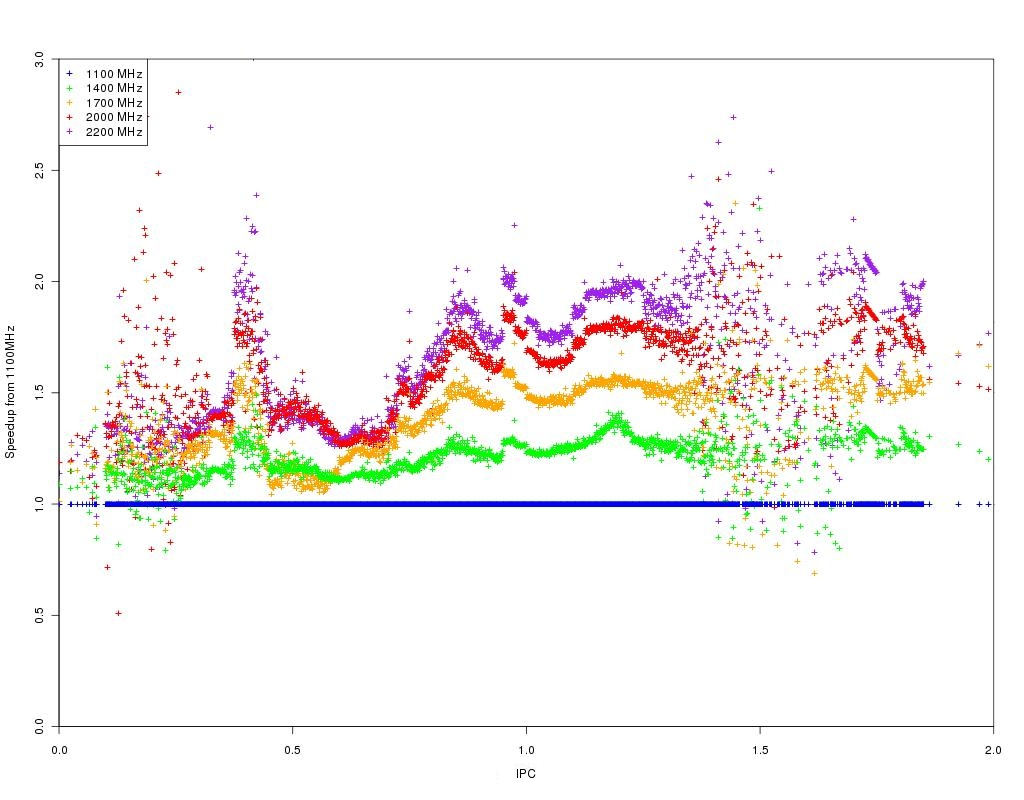
\includegraphics[height=3in]{figures/ipc_speedup.jpg}%}
    \caption{Speedup dependence with IPC}
  \end{center}
  \label{fig:ipc_speedup}
\end{figure}

By reducing clock speed (and hence power consumption), it can be hypothesized that the execution time
increases proportionally and hence maintaining the total energy consumption.
Figure~\ref{fig:ipc_epi} validates this claim that 
the energy consumption per instruction (EPI) is invariant of clock speed, except at lower IPC levels
where lower clock speeds demonstrate better EPI behavior.

\begin{figure}[h!]
  \begin{center}
    %\resizebox{\columnwidth}{!}{
    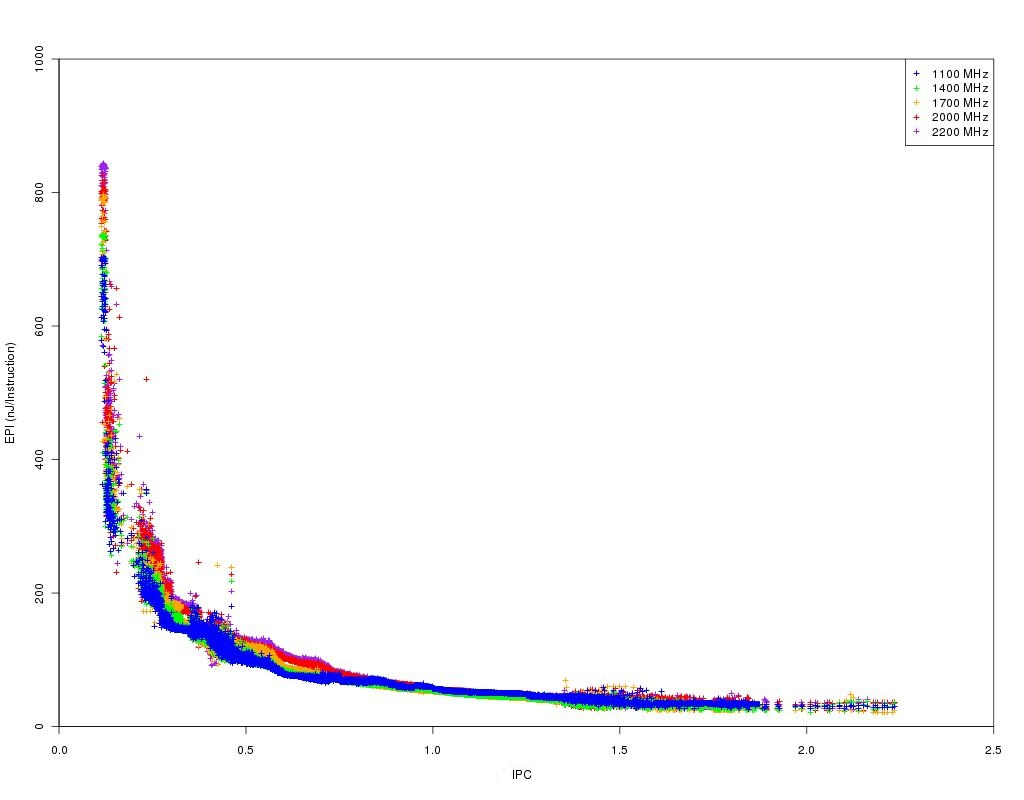
\includegraphics[height=3in]{figures/ipc_epi.jpg}%}
    \caption{Energy consumption per instruction variance with IPC}
    \label{fig:ipc_epi}
  \end{center}
\end{figure}

%%%%%%%%%%%%%%%%%%%%%%%%%%%%%%%%%%%%%%%%%%%%%%%%%%%%%%%%%%%%%%%%%%%%%%%%%%%%%%%
\section{Hierarchical processor organization}~\label{sec:proc_org}
%%%%%%%%%%%%%%%%%%%%%%%%%%%%%%%%%%%%%%%%%%%%%%%%%%%%%%%%%%%%%%%%%%%%%%%%%%%%%%%

Sections \ref{sec:perf_behav} and \ref{sec:quant_perf}  provide a strong motivation to
scale voltage and frequency of processors based on the performance of the workload.
While most of the research pertaining to workload based DVFS direct their attention of changing the voltage and frequency levels
based on the task's demand, none consider the possibility that such a performance state might
already be available on another core which can be remedied by a simple migration without the 
causality of rapid performance state transitions. The motivation to substitute migration to
a frequency transition is further enhanced with the current multi-core race where the probability
of such a situation improves proportionally.  

In order to enable scheduling on asymmetric multiprocessors, the first implementation
step was to organize the processor set as groups with equal performance states. 
The term performance state or P-State will be used to differentiate varied voltage and
frequency configurations which a processor is allowed to have, and is indicated by
$P_{0}$ through $P_{M-1}$ where, $P_0$ is the configuration with the lowest clock speed
and voltage (In effect a lower power consumption). Each set maintains the usage in terms
of actively running tasks in the particular group to enable load balancing between 
groups of varied performance states. This view of the processor set is shown in
Figure~\ref{fig:processor_groups} and mathematically viewed as a vector of sets shown in Figure~\ref{fig:layout_scheduler}.
Here, $C_{P_{i}}$ is the set of processors which are at 
a performance state of $P_{i}$. Individual processor cores are represented as $C_{i}$.


\begin{figure}[h!]
  \begin{center}
%    \resizebox{\columnwidth}{!}{
    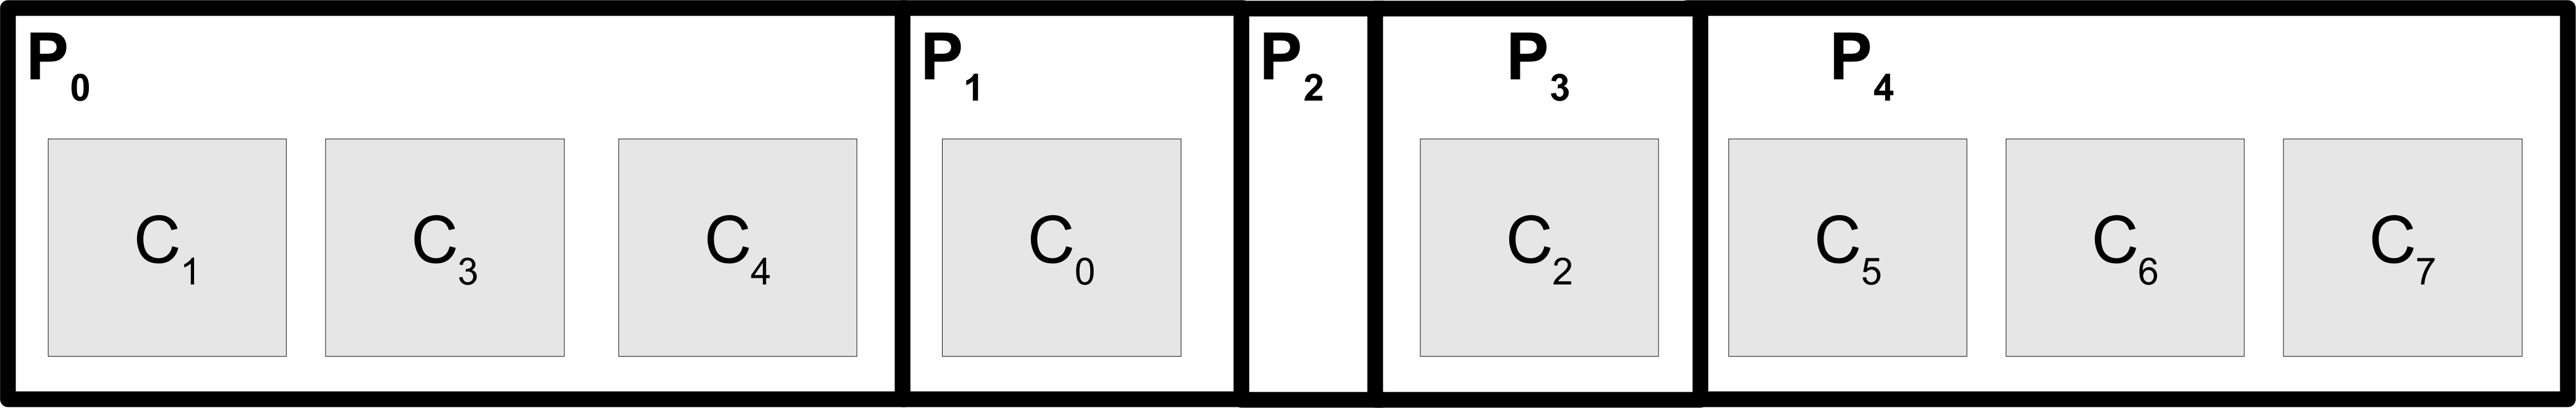
\includegraphics[height=1in]{figures/Processor_Organization.jpg}%}
    \caption{Multi-processor organization}
    \label{fig:processor_groups}
  \end{center}
\end{figure}

\begin{figure}[h!]
\centering
\begin{equation*}
   L^{s} = \left[
     \begin{array}{lccr}
       C_{P_{0}} & C_{P_{1}} & ... & C_{P_{M-1}}
     \end{array} \right]
\end{equation*}
\caption{Definition of the processor layout with M performance states}
\label{fig:layout_scheduler}
\end{figure}


%%%%%%%%%%%%%%%%%%%%%%%%%%%%%%%%%%%%%%%%%%%%%%%%%%%%%%%%%%%%%%%%%%%%%%%%%%%%%%%
\section{Hardware performance counters}~\label{sec:perf_counters}
%%%%%%%%%%%%%%%%%%%%%%%%%%%%%%%%%%%%%%%%%%%%%%%%%%%%%%%%%%%%%%%%%%%%%%%%%%%%%%%

In order to quantitatively measure the performance of each task, 
a driver was developed to read and configure the hardware performance counters
present in the AMD and Intel Architectures. Two counters one to count retired instructions
while another to count real clock cycles were configured to measure the sample IPC 
of an executing workload as shown in Figure~\ref{fig:hw_counters}. Every
request for IPC made to the performance monitoring subsystem, the current value of 
both counters are read, and based on which the IPC is computed and returned to the consumer
as a fixed point value with the lower three bits containing the fraction (a precision 
of 0.125). After every successful transaction, the counters are cleared and continue incrementing with each event.
The performance monitoring subsystem is unaware of the current executing task and it is the scheduler's
responsibility to read the IPC level before switching out tasks form the running state. 

\begin{figure}[h!]
  \begin{center}
    %\resizebox{\columnwidth}{!}{
    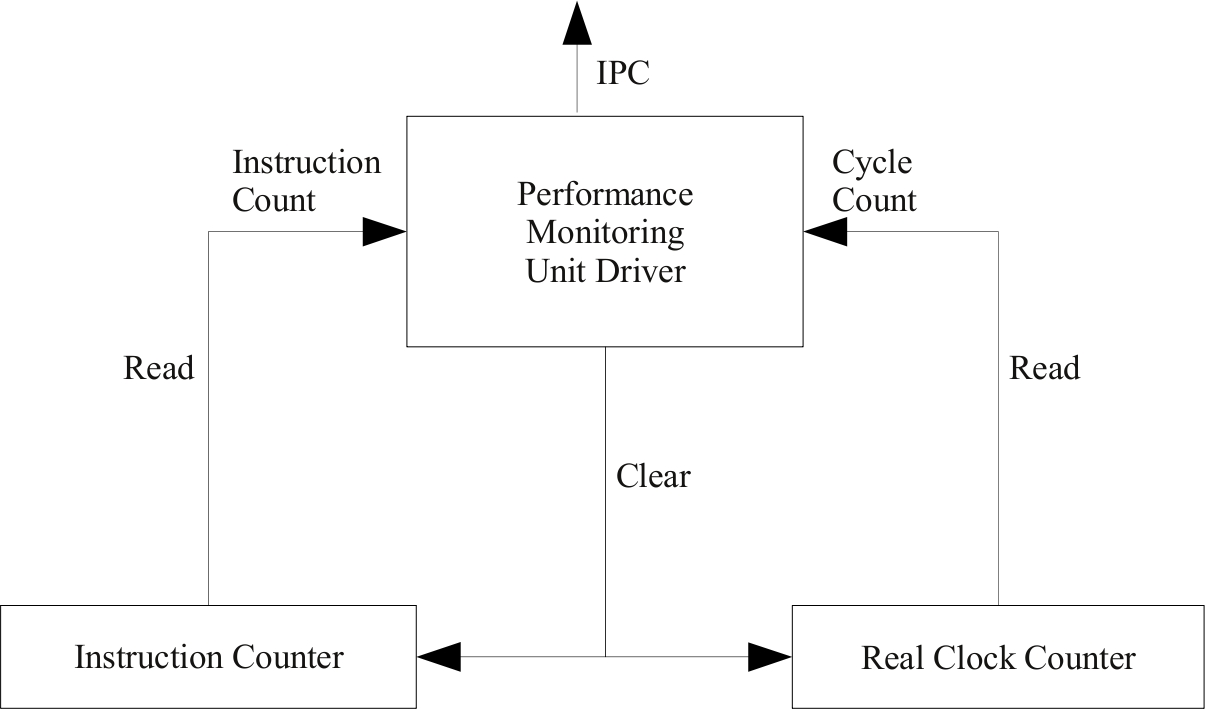
\includegraphics[height=2in]{figures/HW_Counter.jpg}%}
    \caption{Hardware performance monitoring counters}
    \label{fig:hw_counters}
  \end{center}
\end{figure}

%%%%%%%%%%%%%%%%%%%%%%%%%%%%%%%%%%%%%%%%%%%%%%%%%%%%%%%%%%%%%%%%%%%%%%%%%%%%%%%
\section{Scheduling methodology}~\label{sec:pds}
%%%%%%%%%%%%%%%%%%%%%%%%%%%%%%%%%%%%%%%%%%%%%%%ttf-opensymbol%%%%%%%%%%%%%%%%%%%%%%%%%%%%%%%%

It is common for the number of tasks in the ready state to be greater than the total number
of processors. Most time sharing scheduling systems regularly switch out a running task
to another in order to provide fair equal execution times for all tasks. This execution slice is commonly 
referred to as the scheduling quanta. The Linux Scheduling system, in order to support symmetric 
multi-processor environments, maintains separate run-queues
for each processing element. As a direct consequence, the scheduling state diagram is replicated for each processor. 
Migration, a procedure of moving a runnable task from one processor to another is reduced to migrating the task from
one run-queue to another. 

Figure~\ref{fig:pds_method} shows the state diagram of the performance directed scheduler which is a modification of
the default Linux scheduler with an additional pseudo state (Performance directed Migration) introduced at the transition 
away from the running state (This is termed as a pseudo state as it is just a place holder to describe the arcs at 
which performance directed decisions are made). At this state as shown in Figure~\ref{fig:pds_migration}, the hardware 
performance counters are queried for the value of the current IPC (Instructions per clock). 
Based on this quantitative measure of the task's performance,
a mapping from IPC to a required performance state ($P'$) is made. This mapping can potentially be done is a number of ways 
of which two were implemented and evaluated and described in the following two subsections. Once $P'$ is estimated, 
the layout $L^s$ is is queried for the total number of processors in the set $C_{P'}$ and the total number of tasks in the 
ready or running state for processors in $C_{P'}$. If the set $C_{P'}$ is populated or the total number of tasks executing 
on the processors in set $C_{P'}$ is lesser than or equal
to the number of processors in $C_{P'}$, then $P'' = P'$. But if such is not the case, then the layout $L^s$ is searched
for a set $C_{P''}$ such that $P''$ is closest to $P'$, and $C_{P''}$ is populated and the total number of tasks 
executing in the set $C_{P''}$ is lesser than the number of processors in $C_{P''}$. If all fails, then the layout
is searched for a state $P''$ such that $C_{P''}$ is populated and the load (Computed as the total number of tasks 
divided by the number of processors) is minimum. Decisions on the exact processor a task has to execute on is made by the 
underlying native scheduler of the operating system and the PDS is completely oblivious to any further details.
As an interface to the mutator which will be explained in Chapter~\ref{chap:delta}, PDS
increments the cell corresponding to $P'$ in the demand vector \textbf{D} ($D_{P'} = D_{P'} + 1$).

\begin{figure}[h!]
  \begin{center}
%    \resizebox{\columnwidth}{!}{
    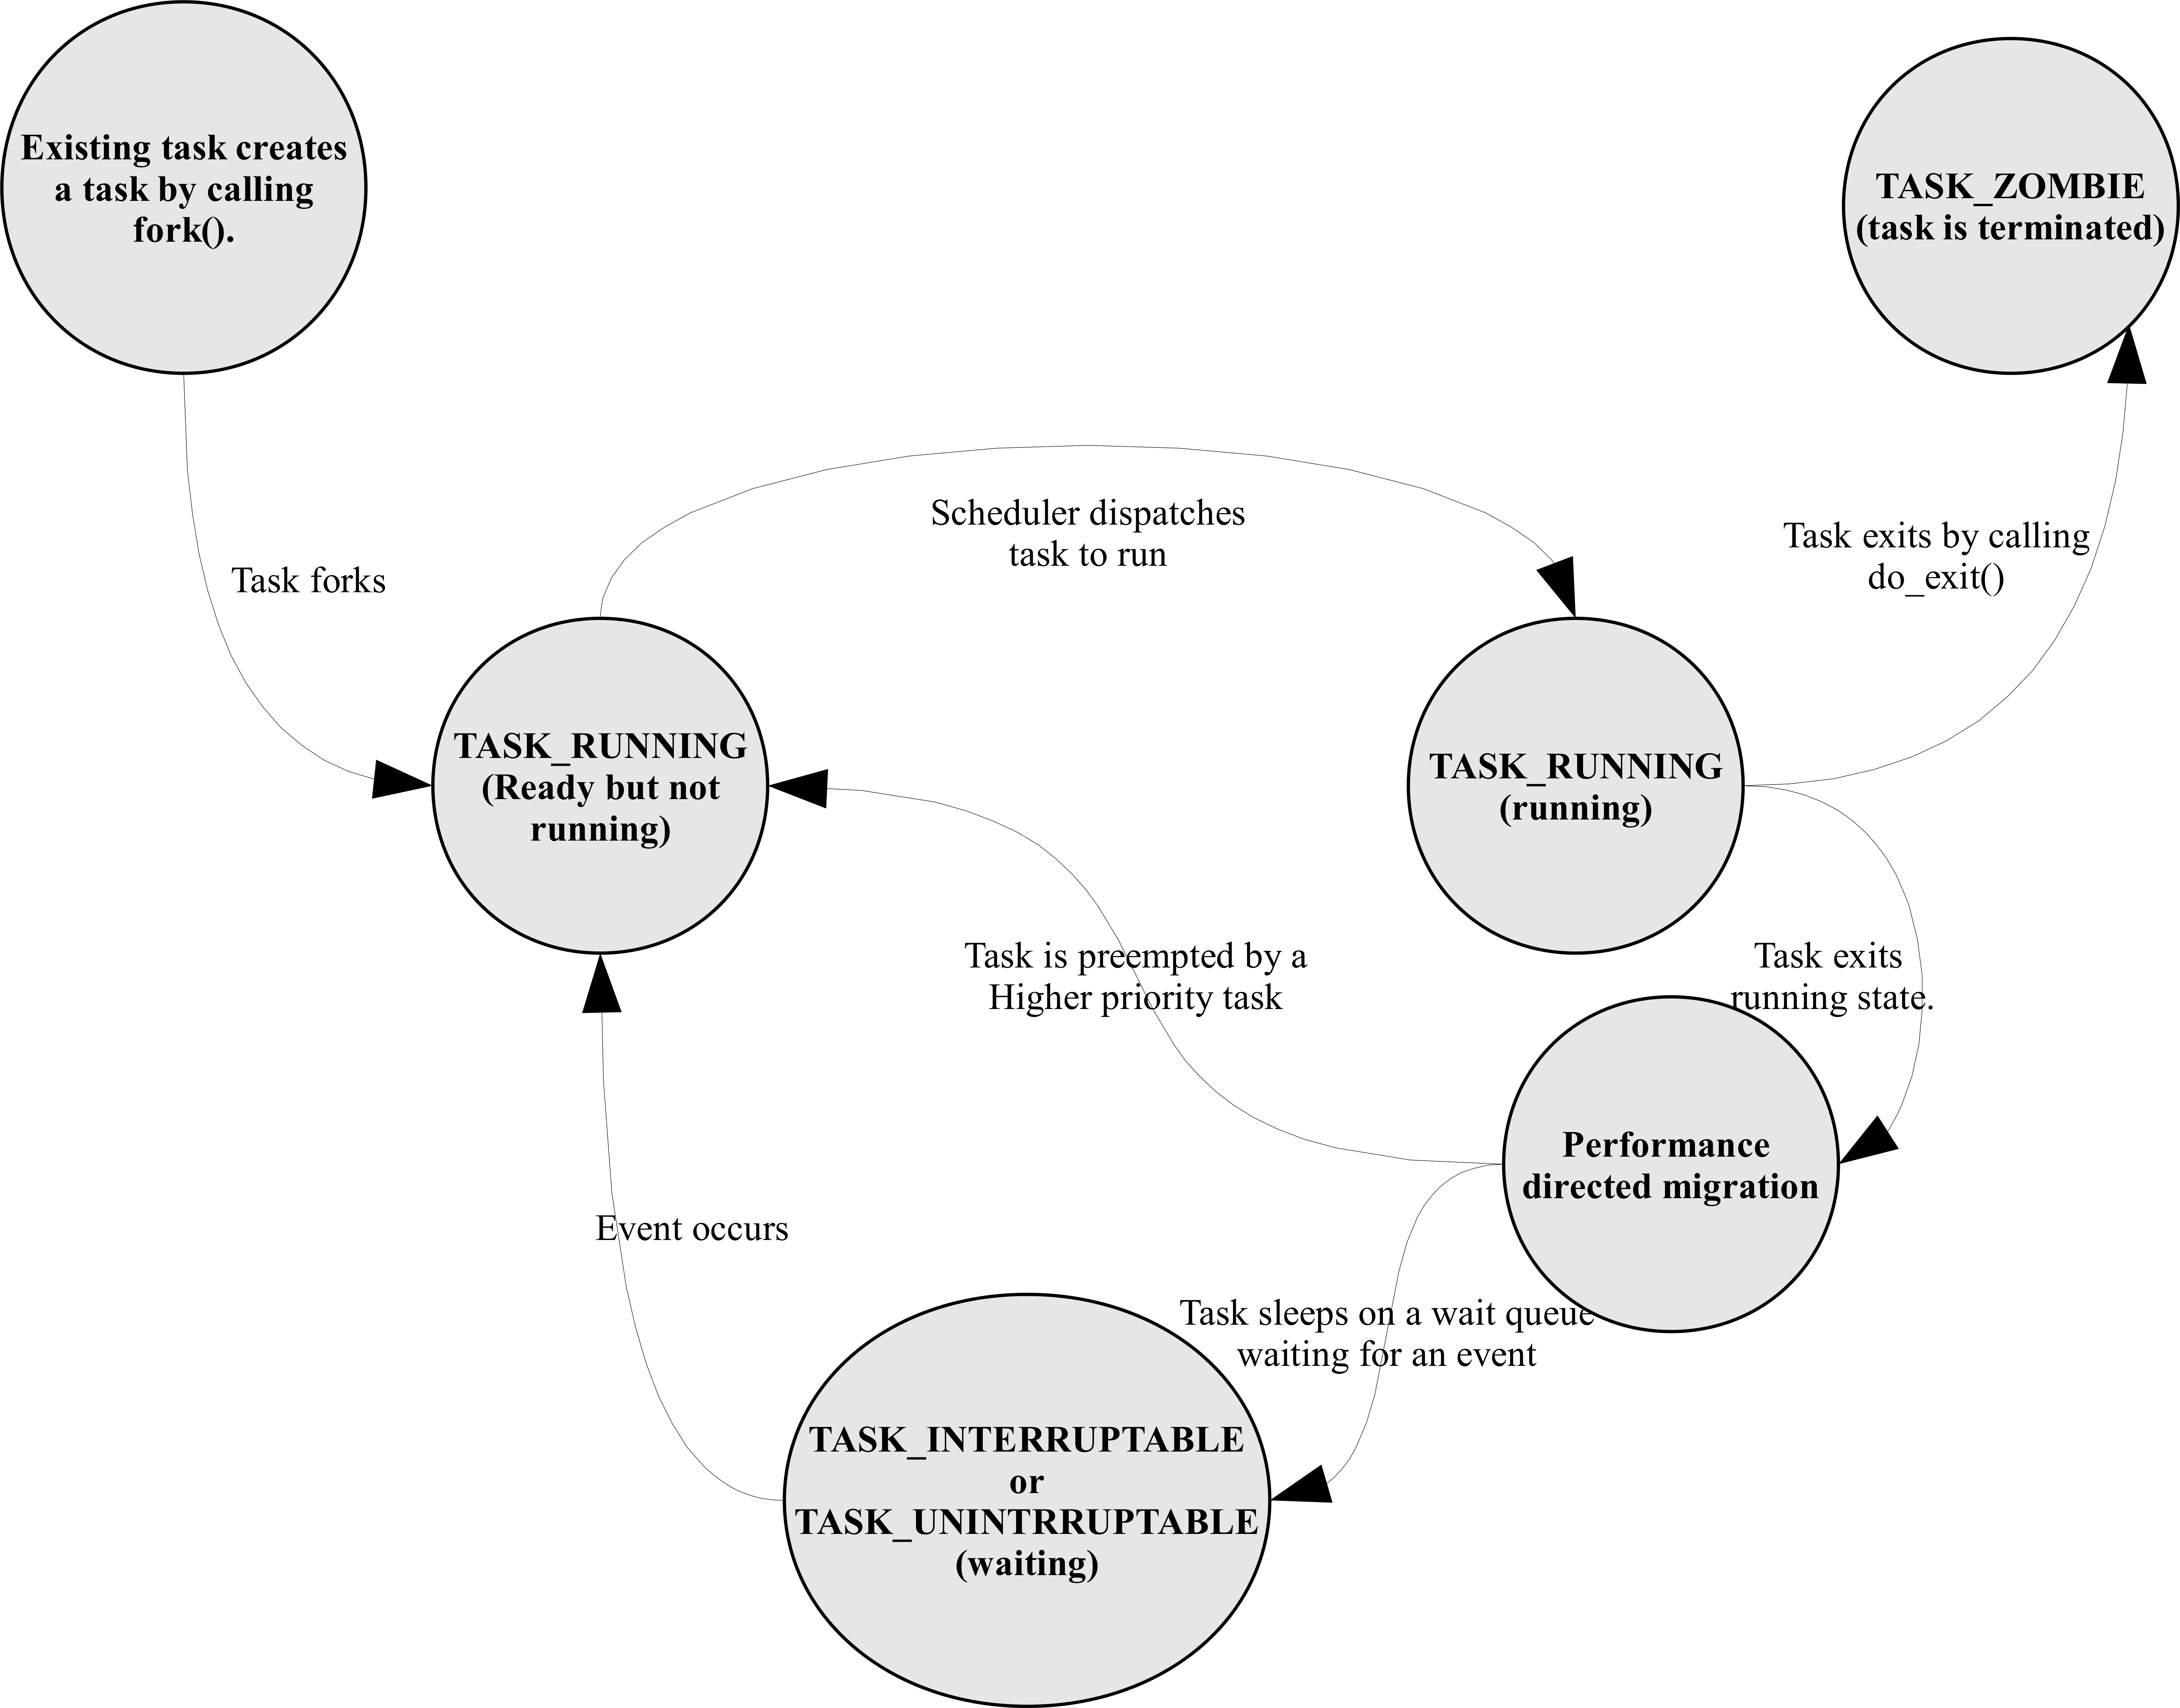
\includegraphics[height=3in]{figures/Mod_Linux_Sched.jpg}%}
    \caption{Scheduling state diagram}
    \label{fig:pds_method}
  \end{center}
\end{figure}

\begin{figure}[h!]
  \begin{center}
    \resizebox{\columnwidth}{!}{
    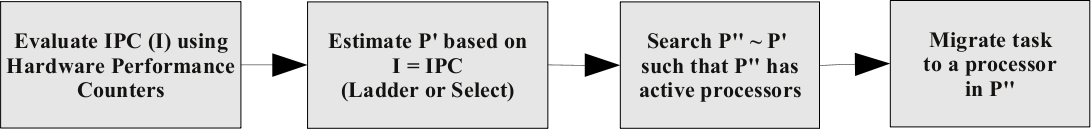
\includegraphics{figures/Migration.jpg}}
    \caption{Performance directed migration}
    \label{fig:pds_migration}
  \end{center}
\end{figure}


%%%%%%%%%%%%%%%%%%%%%%%%%%%%%%%%%%%%%%%%%%%%%%%%%%%%%%%%%%%%%%%%%%%%%%%%%%%%%%%
\subsection{Ladder performance state estimation}~\label{sec:ladder}
%%%%%%%%%%%%%%%%%%%%%%%%%%%%%%%%%%%%%%%%%%%%%%%%%%%%%%%%%%%%%%%%%%%%%%%%%%%%%%%

The ladder performance state estimation sports a simple decision procedure. If $IPC > H$ 
where \textbf{H} is set to 0.875, then $P'$ is chosen such that is is higher than the state
at which the task is currently executing with ($P' = P + 1$). If $IPC < L$ ($L = 0.5$), then 
$P'$ is chosen to be one less than the state at which the task is executing with ($P' = P - 1$). 
Otherwise the $P'$ is chosen to be equal to $P$. The advantage of the procedure is the lower
choice (two: H and L) available to the system administrator. It is clear that the wrong choice of these
thresholds can cause undesirable power and performance behavior of the system. These thresholds are
selected based on the graph shown in Figure~\ref{fig:ipc_speedup}. 

\begin{figure}[h!]
  \begin{center}
%    \resizebox{\columnwidth}{!}{
    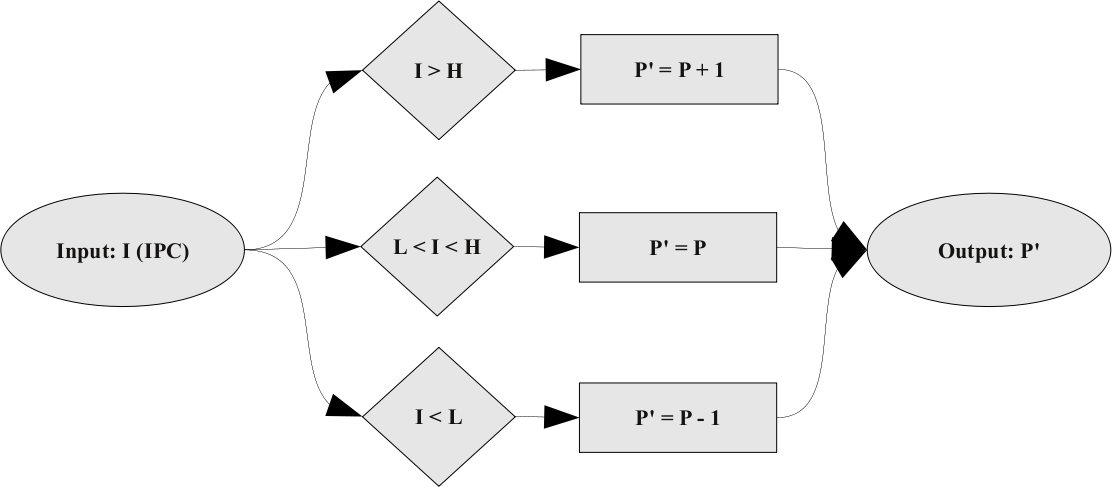
\includegraphics[height=2in]{figures/Ladder_Evaluation.jpg}%}
    \caption{Ladder performance state estimation algorithm}
    \label{fig:ladder_method}
  \end{center}
\end{figure}

%%%%%%%%%%%%%%%%%%%%%%%%%%%%%%%%%%%%%%%%%%%%%%%%%%%%%%%%%%%%%%%%%%%%%%%%%%%%%%%
\subsection{Select performance state estimation}~\label{sec:select}
%%%%%%%%%%%%%%%%%%%%%%%%%%%%%%%%%%%%%%%%%%%%%%%%%%%%%%%%%%%%%%%%%%%%%%%%%%%%%%%

A logical extension of the ladder estimation, is the select estimation shown in Figure~\ref{fig:select_method}.
This is when, a performance state is fixed for each range of IPC. Such a system was implemented with 
threshold values shown in Table~\ref{tab:sel_threshold}. This system was evaluated along with
the ladder evaluation with the delta based mutation described in Chapter~\ref{chap:delta}.

\begin{figure}[h!]
  \begin{center}
%    \resizebox{\columnwidth}{!}{
    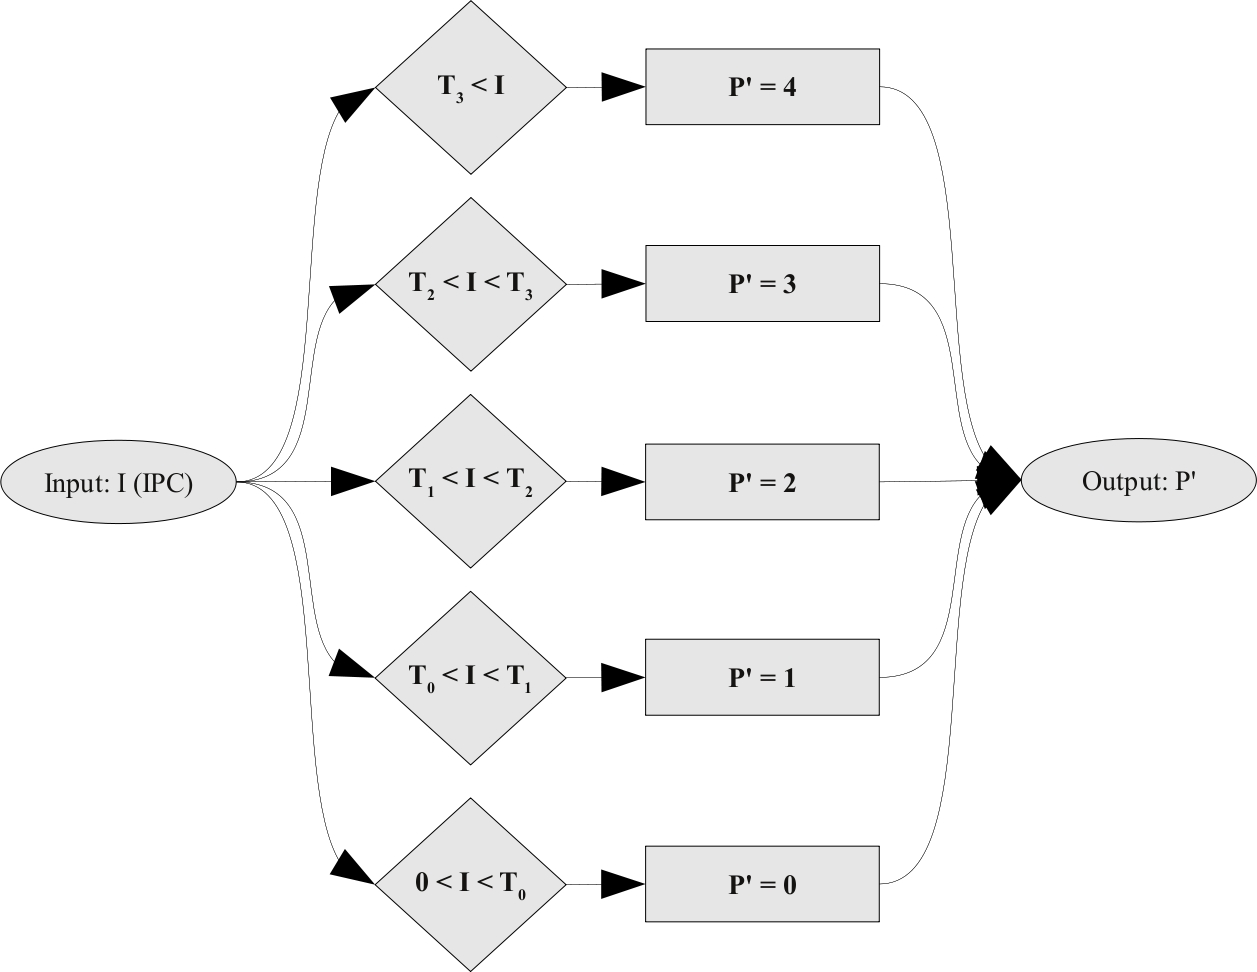
\includegraphics[height=3in]{figures/Select_Evaluation.jpg}%}
    \caption{Select performance state estimation algorithm}
    \label{fig:select_method}
  \end{center}
\end{figure}

\begin{table}[h!]
 \begin{center}
\begin{tabular}{| l | l | }
\hline	
Threshold & Value \\
\hline
$T_0$ & 0.25  \\
$T_1$ & 0.50  \\
$T_2$ & 0.75  \\
$T_3$ & 1.25  \\
\hline  
\end{tabular}
 \end{center}
\caption{Threshold values for the select evaluation}
\label{tab:sel_threshold}
\end{table}


%%%%%%%%%%%%%%%%%%%%%%%%%%%%%%%%%%%%%%%%%%%%%%%%%%%%%%%%%%%%%%%%%%%%%%%%%%%%%%%
\section{Experimental setup}~\label{sec:pds_exp}
%%%%%%%%%%%%%%%%%%%%%%%%%%%%%%%%%%%%%%%%%%%%%%%%%%%%%%%%%%%%%%%%%%%%%%%%%%%%%%%

The experiments were conducted on a AMD quad-core Barcelona which allows individual
processor cores to be set to different clock speeds. Different synthetic workloads
based on real world usages were set up using the SPEC2006 benchmarks and classified based on their IPC. The 
individual members of each group are provided in Appendix~\ref{app:benchmark}. The workload was started
on the layouts provided in Table~\ref{tab:proc_layouts}, and the execution time of each
member benchmark was measured and summed to arrive at a single execution time per 
workload. The experiment was repeated multiple times and the mean of the execution times were 
compared with that of the $[4,4,4,4]$ layout to get the percentage slow down. 
The results are shown in Figure~\ref{fig:fixed_res}.  

\begin{table}[h!]
 \begin{center}
\begin{tabular}{| l | l | l | l | l | }
\hline	
Layout Name & $P_{C_{0}}$ & $P_{C_{1}}$ & $P_{C_{2}}$ & $P_{C_{3}}$ \\
\hline
a & 0 & 0 & 0 & 0 \\
b & 0 & 0 & 1 & 1 \\
c & 0 & 0 & 2 & 2 \\
d & 0 & 0 & 0 & 4 \\
e & 1 & 1 & 2 & 2 \\
f & 0 & 0 & 3 & 3 \\
g & 0 & 0 & 4 & 4 \\
h & 1 & 1 & 3 & 3 \\
i & 1 & 1 & 4 & 4 \\
j & 2 & 2 & 3 & 3 \\ 
k & 2 & 2 & 4 & 4 \\ 
l & 0 & 4 & 4 & 4 \\
m & 3 & 3 & 4 & 4 \\
n & 4 & 4 & 4 & 4 \\
\hline  
\end{tabular}
 \end{center}
\caption{Experimental layouts}
\label{tab:proc_layouts}
\end{table}

\begin{figure}[h!]
  \begin{center}
    %\resizebox{\columnwidth}{!}{
    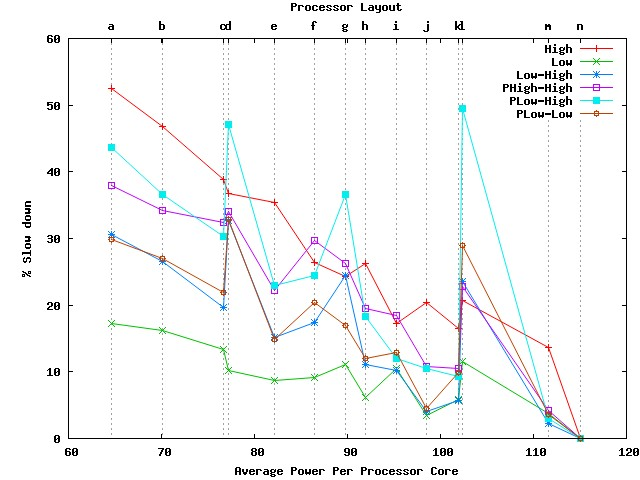
\includegraphics[height=4in]{figures/fixed_results.jpg}%}
    \caption{Slowdown vs power consumption for fixed layouts}
    \label{fig:fixed_res}
  \end{center}
\end{figure}

One obvious trend is decrease in the percentage slowdown with the increase of power provided per 
core (Higher performance states available)
increases. The problem with fixed static layouts are obvious from the peaks observed
whenever there is an asymmetry in the layout for example $[0,0,0,4]$ where processor
$C_3$ is in state $P_4$ while the remaining processors $C_0$,$C_1$ and $C_2$ are in
$P_0$. A particular time line for such a configuration is shown in Figure~\ref{fig:fight_to_death}.
The reason for the spikes become fairly obvious from the rapid migrations observed for
a fairly stable phased behavior. This is usually common when there are more tasks battling
over a lower number of processors where the time spent in migrations
become noticeable and add to the slow down of the task. 



\begin{figure}[h!]
  \begin{center}
    %\resizebox{\columnwidth}{!}{
    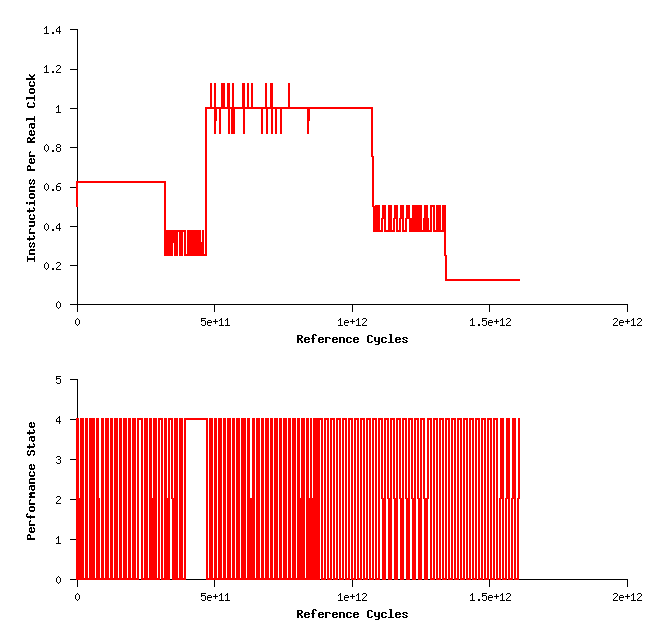
\includegraphics[height=3in]{figures/astar_fight.png}%}
    \caption{Astar running on a $[0,0,0,4]$ layout}
    \label{fig:fight_to_death}
  \end{center}
\end{figure}

%%%%%%%%%%%%%%%%%%%%%%%%%%%%%%%%%%%%%%%%%%%%%%%%%%%%%%%%%%%%%%%%%%%%%%%%%%%%%%%
\chapter{Power-aware throughput management on multi-core systems}~\label{chap:delta}
%%%%%%%%%%%%%%%%%%%%%%%%%%%%%%%%%%%%%%%%%%%%%%%%%%%%%%%%%%%%%%%%%%%%%%%%%%%%%%%

Power management systems have to look at two facets: Power and energy. Servers are
usually limited to the amount of peak power and energy
consumed in order to reduce maintenance cost. Power and energy considerations more often than not, accounts 
to the reduction in server space expansion in industries. To combat these constraints, power management systems
are becoming increasingly common in the server space which were previously restricted for mobile devices.
Two common methodologies exist to reduce the power consumption of a compute element. The first among which
is to turn off (and hence reduce the power consumption to the orders of milliwatts) processors during idle time. 
The second is to lower the operating frequency and voltage of the processor at idle or active time to observe
a proportionally lower power consumption.
In order to fully utilize server nodes and minimize idle time, the current trend among industries is to 
run multiple \textit{virtual machines} on a single server rack thus making varied workloads common place
in an otherwise single purpose server usage. This element further enhances the requirement of 
dynamic non-trace driven power management systems. \cite{VirtualPower} discusses a power optimizer specialized
for a virtual machine farm, but fail to recognize the workload characteristics of these systems.

Lowering frequency has a pleasant benefit of reducing the power consumption and hence
the energy and cooling costs. But as shown in Chapter~\ref{chap:pds}, Figures~\ref{fig:ipc_speedup} 
and \ref{fig:ipc_epi}, when the average IPC of an application is high, reduction in 
frequency only causes the application to execute for a proportionally longer duration and 
hence having no energy benefit (Figure~\ref{fig:ipc_epi}). The only advantage of reducing
the frequency is the reduction of energy supply into the system per unit time and hence
possibly lower heat dissipation. 

Some power management systems such as \cite{OnDemand} manipulate the DVFS (dynamic voltage and freqency) configuration
of the system based on the load. The primary problem with such approaches are not in
their implementation or design, but the fact that there are better power management
systems where the entire processor is powered down during idle time whose power savings are considerably higher than DVFS. 
This brings us to utilizing DVFS mechanisms to conserve power during system \textit{active}
state. 

\cite{AnIntraTask}, \cite{LiveRuntime} and \cite{Phaseaware} propose adapting the clock speed of the the processing element based
on the current application's demand. All these methodologies assumes the fact that DVFS transitions
are local to that processor core. Some multi-core processors have dependency between 
processor cores (transitioning one might potentially transition the other) or systems with 
symmetric multi-threaded features where a single processor
core is visible to the operating system as multiple virtual processors. Thus, applications
executing on such processing elements are tied to each other and any DVFS
transition based on one application might potentially affect another negatively. 
Chapter~\ref{chap:pds} showed that such transitions could be remedied with a simple processor migration
requiring power optimizers to react to the needs of a scheduler.

%%%%%%%%%%%%%%%%%%%%%%%%%%%%%%%%%%%%%%%%%%%%%%%%%%%%%%%%%%%%%%%%%%%%%%%%%%%%%%%
\section{Common power management systems}~\label{sec:common_pow}
%%%%%%%%%%%%%%%%%%%%%%%%%%%%%%%%%%%%%%%%%%%%%%%%%%%%%%%%%%%%%%%%%%%%%%%%%%%%%%%

The most popular among power management techniques are load directed systems
which transition a processor to a higher or lower performance state based on it's current load. Two
of these techniques: \textit{ondemand}\cite{OnDemand} and \textit{conservative} 
were simulated within the existing infrastructure. The \textit{ondemand}
system raises the performance state to the highest possible level at high loads, and
reduces the performance state gradually to the lowest state during lower load.
The \textit{conservative}
system gradually changes the performance state in either direction. These two are 
shown in Figures \ref{fig:math_ondemand} and \ref{fig:math_conservative}. As both 
are similar in design, only the \textit{ondemand} system was heavily analyzed 
along with the proposed power management systems.

\begin{figure}[h!]
\centering
\begin{equation*}
    P_{i}' = \left\{ \begin{array}{lr} 
                   P_{M-1} & : Load \geq 0.8 \\
		   P_{i}-1 & : Load < 0.8
                  \end{array} \right.
\end{equation*}
\caption{The ondemand power management system with M performance states}
\label{fig:math_ondemand}
\end{figure}

\begin{figure}[h!]
\centering
\begin{equation*}
    P_{i}' = \left\{ \begin{array}{lr} 
                   P_{i}+1 & : Load \geq 0.8 \\
		   P_{i}-1 & : Load < 0.8
                  \end{array} \right.
\end{equation*}
\caption{The conservative power management system with M performance states}
\label{fig:math_conservative}
\end{figure}

%%%%%%%%%%%%%%%%%%%%%%%%%%%%%%%%%%%%%%%%%%%%%%%%%%%%%%%%%%%%%%%%%%%%%%%%%%%%%%%
\section{Overview of the Linux cpufreq architecture}~\label{sec:cpufreq}
%%%%%%%%%%%%%%%%%%%%%%%%%%%%%%%%%%%%%%%%%%%%%%%%%%%%%%%%%%%%%%%%%%%%%%%%%%%%%%%

In order to maintain architecture independence, separation of methodology 
and policy, the subsystem in the Linux kernel responsible for managing the 
voltage and frequency configuration separates the procedure into three layers. \textit{cpufreq-drivers}
are responsible for the actual P-State transition and register with the 
intermediate \textit{cpufreq} layer. \textit{cpufreq-governors} are responsible for
policy (How and when to initiate a transition) and also register with the 
\textit{cpufreq} layer. Once a working configuration is initialized, the 
\textit{cpufreq-governor} instructs the \textit{cpufreq-driver} in an indirect
fashion on the required transition. As most of the experimentation mentioned in
this text relates to the AMD Barcelona, the \textit{powernow-k8} \textit{cpufreq-driver}
was used to initiate the transition. 

A \textit{cpufreq} governor \textit{seeker}
was developed having kernel exported interfaces for the mutator to request transitions. 
A simple registration method was introduced to allow the mutator to be informed 
every time a transition is complete as shown in Figure~\ref{fig:governor}. 
The asynchronous call back mechanism allows the mutator to
update its data structures even when an entity other than itself ( For example, through
the \textit{sysfs} interface) requests for a performance state change. 

\begin{figure}[h!]
  \begin{center}
    %\resizebox{\columnwidth}{!}{
    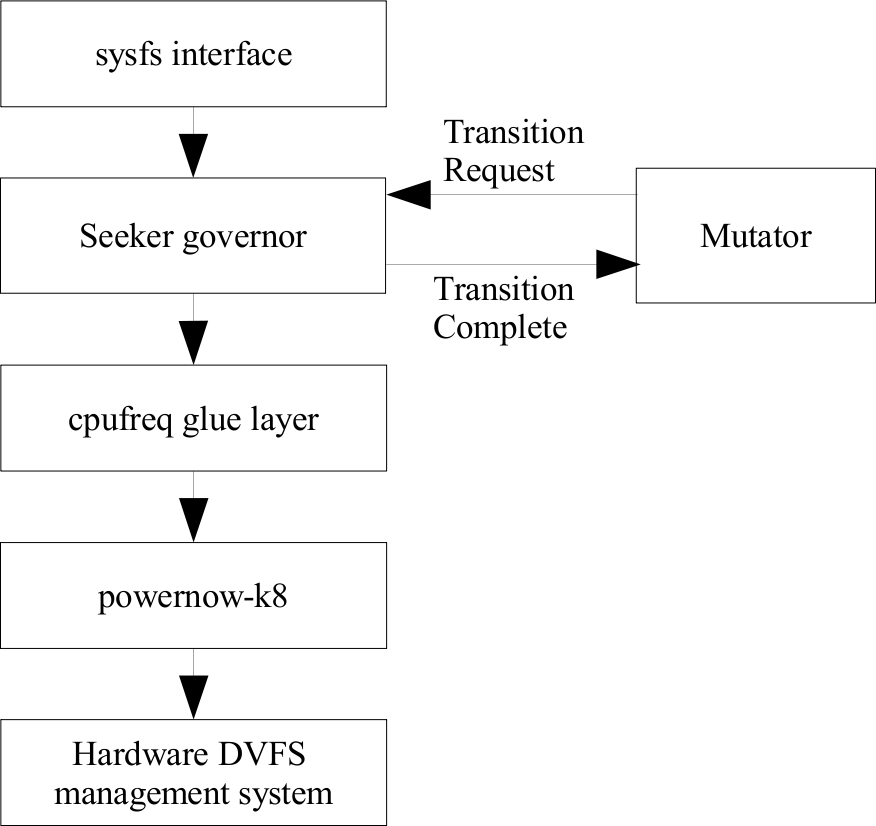
\includegraphics[height=2in]{figures/seeker_governor.jpg}%}
    \caption{The Seeker governor}
    \label{fig:governor}
  \end{center}
\end{figure}

%%%%%%%%%%%%%%%%%%%%%%%%%%%%%%%%%%%%%%%%%%%%%%%%%%%%%%%%%%%%%%%%%%%%%%%%%%%%%%%
\section{Defining the processor layout}~\label{sec:layout}
%%%%%%%%%%%%%%%%%%%%%%%%%%%%%%%%%%%%%%%%%%%%%%%%%%%%%%%%%%%%%%%%%%%%%%%%%%%%%%%

The mutator maintains the layout of the processors $L^m$ as shown in Equation~\eqref{eq:mutator_layout_view}
where N is the total number of processors and 
$P_{C_{i}}$ is the performance state at which processor i is currently in. 
\begin{equation}
    L^m = [ P_{C_{0}} P_{C_{1}} ... P_{C_{N-1}} ]
\label{eq:mutator_layout_view}
\end{equation}

$L^m$ is a vector of length \textit{N} where each element represents the performance state
of the corresponding processor. 
One view of the layout vector $L^s$ was described in Chapter~\ref{chap:pds} 
which was more optimized to view the system of processors as a hierarchal organization
based on their current performance state as the scheduler is designed to be oblivious to individual processors. 
It is clear that both $L^s$ and $L^m$ are different views of the same information and 
the mutator is solely responsible for keeping both consistent. For the rest of this chapter
references to layout or $L$ are with respect to $L^m$. 


%%%%%%%%%%%%%%%%%%%%%%%%%%%%%%%%%%%%%%%%%%%%%%%%%%%%%%%%%%%%%%%%%%%%%%%%%%%%%%%
\section{The delta constraint}~\label{sec:delta_constraint}
%%%%%%%%%%%%%%%%%%%%%%%%%%%%%%%%%%%%%%%%%%%%%%%%%%%%%%%%%%%%%%%%%%%%%%%%%%%%%%%


It is well known that rapid DVFS transitions can affect the reliability of the system \cite{ImpactDVFS}.
Based on system with a scheduling frequency of \textit{Q} Hz
and \textit{N} processor cores, a per-task demand based DVFS system may potentially cause $Q \times N$ 
DVFS transitions per second. Moore's law predicts the doubling of processor cores every 18 months, implying
future architectures are imposed a linear growth of reliability issues and failure rates with per-task
demand based DVFS systems as proposed in \cite{LiveRuntime} and \cite{Phaseaware}. 

The delta constrained mutation scheme was developed providing the ability to control the rate of transitions
by one, limiting DVFS transitions to be performed globally and at fixed interval lengths termed the mutation
interval. Second, by limiting the magnitude of mutation thus eliminating rapid transitions.
Figure~\ref{fig:schedule_mutate} shows the interaction times of these methods. 
The PDS as described in Chapter~\ref{chap:pds} is performed at the resolution of a scheduler quanta, while
the DVFS transitions are performed at a resolution of the mutation interval. In order to have an absolute
upper bound on the DVFS transitions, a parameter called the delta constraint ($\Delta$) was introduced
which limits the maximum number of mutations which can be performed at any particular instant (And hence
limiting the maximum mutations per second to $\frac{\Delta}{\text{Mutation Interval}}$). 

\begin{figure}[h!]
  \begin{center}
    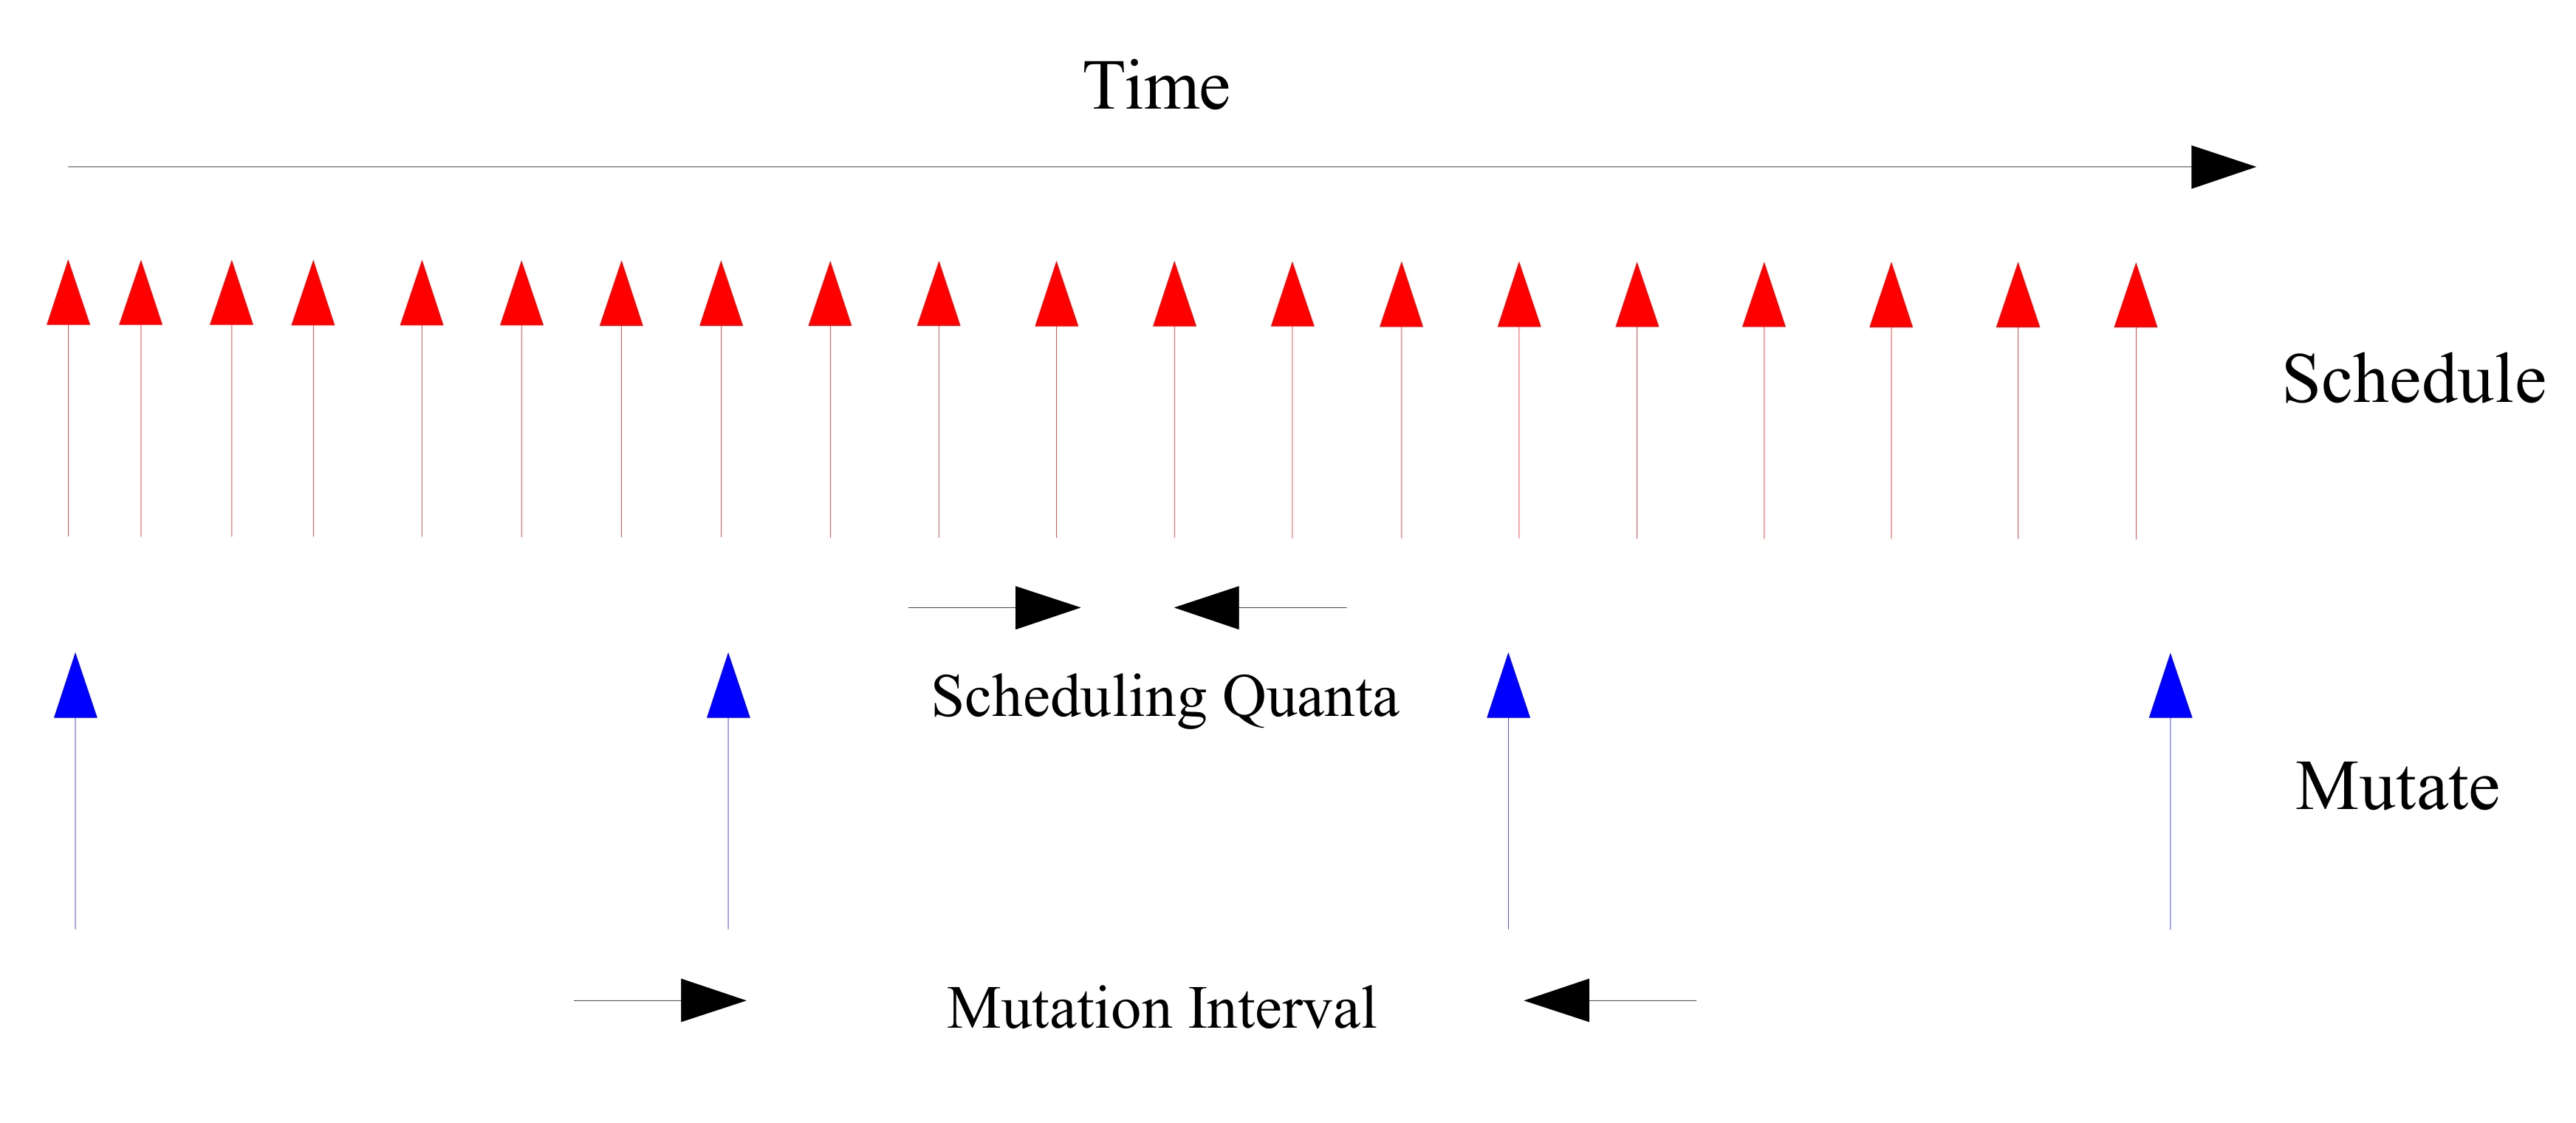
\includegraphics[height=2in]{figures/Schedule_Mutate.jpg}
    \caption{Hypothetical time line displaying the invocation frequencies of the scheduler and the mutator}
    \label{fig:schedule_mutate}
  \end{center}
\end{figure}


Delta ($\Delta$) for a system with \textit{N} processors where each processor \textit{i} is transitioned
from performance state $P_{i}$ to $P_{i}'$ can be defined as shown below in Equation~\eqref{eq:Delta_def}
\begin{equation}
    \Delta \geq \displaystyle\sum_{i=0}^{N-1} {| P_{i} - P_{i}' |}
\label{eq:Delta_def}
\end{equation}
and can also be defined as the Manhattan distance between the layout vector $L$ before the transition and 
the layout vector $L'$ after the transition. Thus the example mutation as shown in Figure~\ref{fig:ex_mutation}
is allowed only for a system with a delta constraint $\Delta \geq 3$. 

\begin{figure}[h!]
  \begin{center}
    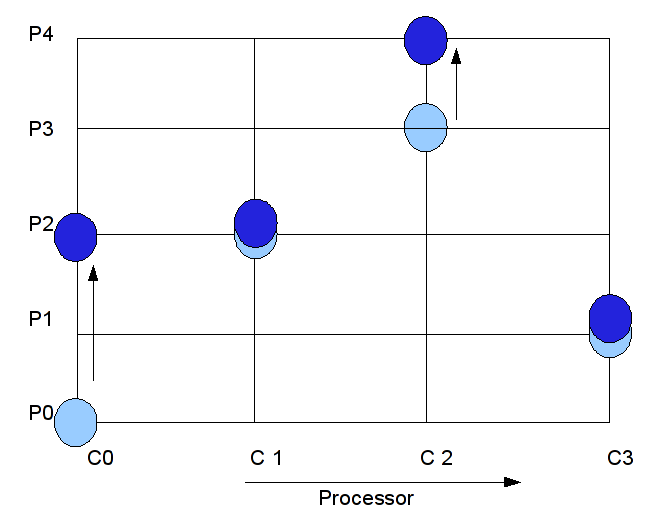
\includegraphics[height=2in]{figures/example_mutation_3.png}
    \caption{Example mutation}
    \label{fig:ex_mutation}
  \end{center}
\end{figure}



%%%%%%%%%%%%%%%%%%%%%%%%%%%%%%%%%%%%%%%%%%%%%%%%%%%%%%%%%%%%%%%%%%%%%%%%%%%%%%%
\section{Problem definition}~\label{sec:ago}
%%%%%%%%%%%%%%%%%%%%%%%%%%%%%%%%%%%%%%%%%%%%%%%%%%%%%%%%%%%%%%%%%%%%%%%%%%%%%%%

An overview of the system required is as follows:
\begin{enumerate}
\item The scheduler estimates the required performance state for each task and maintains the demand, 
a monotonically increasing count, representing the number of times each state was requested. 
\item Each processor can take performance states from $0$ to $M-1$. 
\item The total movements: the Manhattan distance from the current layout to the next layout 
should always be less than or equal to the delta constraint ($\Delta$). 
\item The system should be partial to maintaining a processors current performance state if such a performance state is requested.
\end{enumerate}

This problem can be expressed as a Multiple choice knapsack problem as shown in Figure~\ref{fig:mckp}, where the capacity of the knapsack 
is equal to the delta constraint. Each processor being a variable and multiple choices being the states 
a processor can take. The weight for each choice is the distance that state is from the current 
performance state of the processor. It is well understood that such problems are considered NP-Hard.

\begin{figure}[h!]
\centering
\begin{align*}
    & max \displaystyle\sum_{i=0}^{N-1} \displaystyle\sum_{j=0}^{M-1} d_jx_{ij} \\
    & \text{Subject to} : \displaystyle\sum_{i=0}^{N-1} \displaystyle\sum_{j=0}^{M-1} |L_i - j| x_{ij} \leq \delta \\
    & \displaystyle\sum_{j=0}^{M-1} x_{ij} = 1 , i = 0, 1, ..., N-1 \\
    & x_{ij} \in \{0,1\} , i = 0,1,2,...,N-1 ; j = 0,1,2,...,M-1  
\end{align*}
\caption{Problem with N processors each having M states expressed as a multiple choice knapsack problem}
\label{fig:mckp}
\end{figure}

The algorithm provided in \cite{mckp} was implemented and it soon became obvious 
that the algorithm was inefficient for having no concept of transition direction. Thus for 
a delta constraint of 1, if 
the first 3 processors of a quad core system are at state 0 (The lowest performance state),
while the remaining processor is at state 4 (The highest performance state) and the scheduler
demands all the processors to be at state 3: The dynamic programming approach depicted in
\cite{mckp} will transition the forth processor from state 4 to 3 rather than transition 
one of the lower processors closer to state 3. This unfortunately was just one of the examples
among many when the system did not work. This motivated the development of an iterative 
direction based greedy algorithm described below.


%%%%%%%%%%%%%%%%%%%%%%%%%%%%%%%%%%%%%%%%%%%%%%%%%%%%%%%%%%%%%%%%%%%%%%%%%%%%%%%
\section{The delta constrained mutation algorithm}~\label{sec:delta_algo}
%%%%%%%%%%%%%%%%%%%%%%%%%%%%%%%%%%%%%%%%%%%%%%%%%%%%%%%%%%%%%%%%%%%%%%%%%%%%%%%

Figure~\ref{fig:mutation_algo} describes the steps involved in the iterative greedy algorithm. 
Each sub step is described in further sections. The initialization procedure is described in Section~\ref{sec:mut_init}.
Based on the iteration delta constraint $\delta$, a matrix, Manhattan
matrix (\textbf{S}) is constructed and described in Section~\ref{sec:delta_matrix}.
The Manhattan weight vector \textbf{W} is described in Section~\ref{sec:weight}.
The cooperative demand transformation (Creation of the demand field) is described in
\ref{sec:field}. The greedy winning state \textit{w} selection is described in Section~\ref{sec:winner_state}.
The selection of the processor \textit{c} to transition to the winning state \textit{w} 
is described in Section~\ref{sec:winner_proc}. Finally, the parameter adjustments and iteration
termination conditions are described in Section~\ref{sec:param_adjust}. 

\begin{figure}[h!]
  \begin{center}
    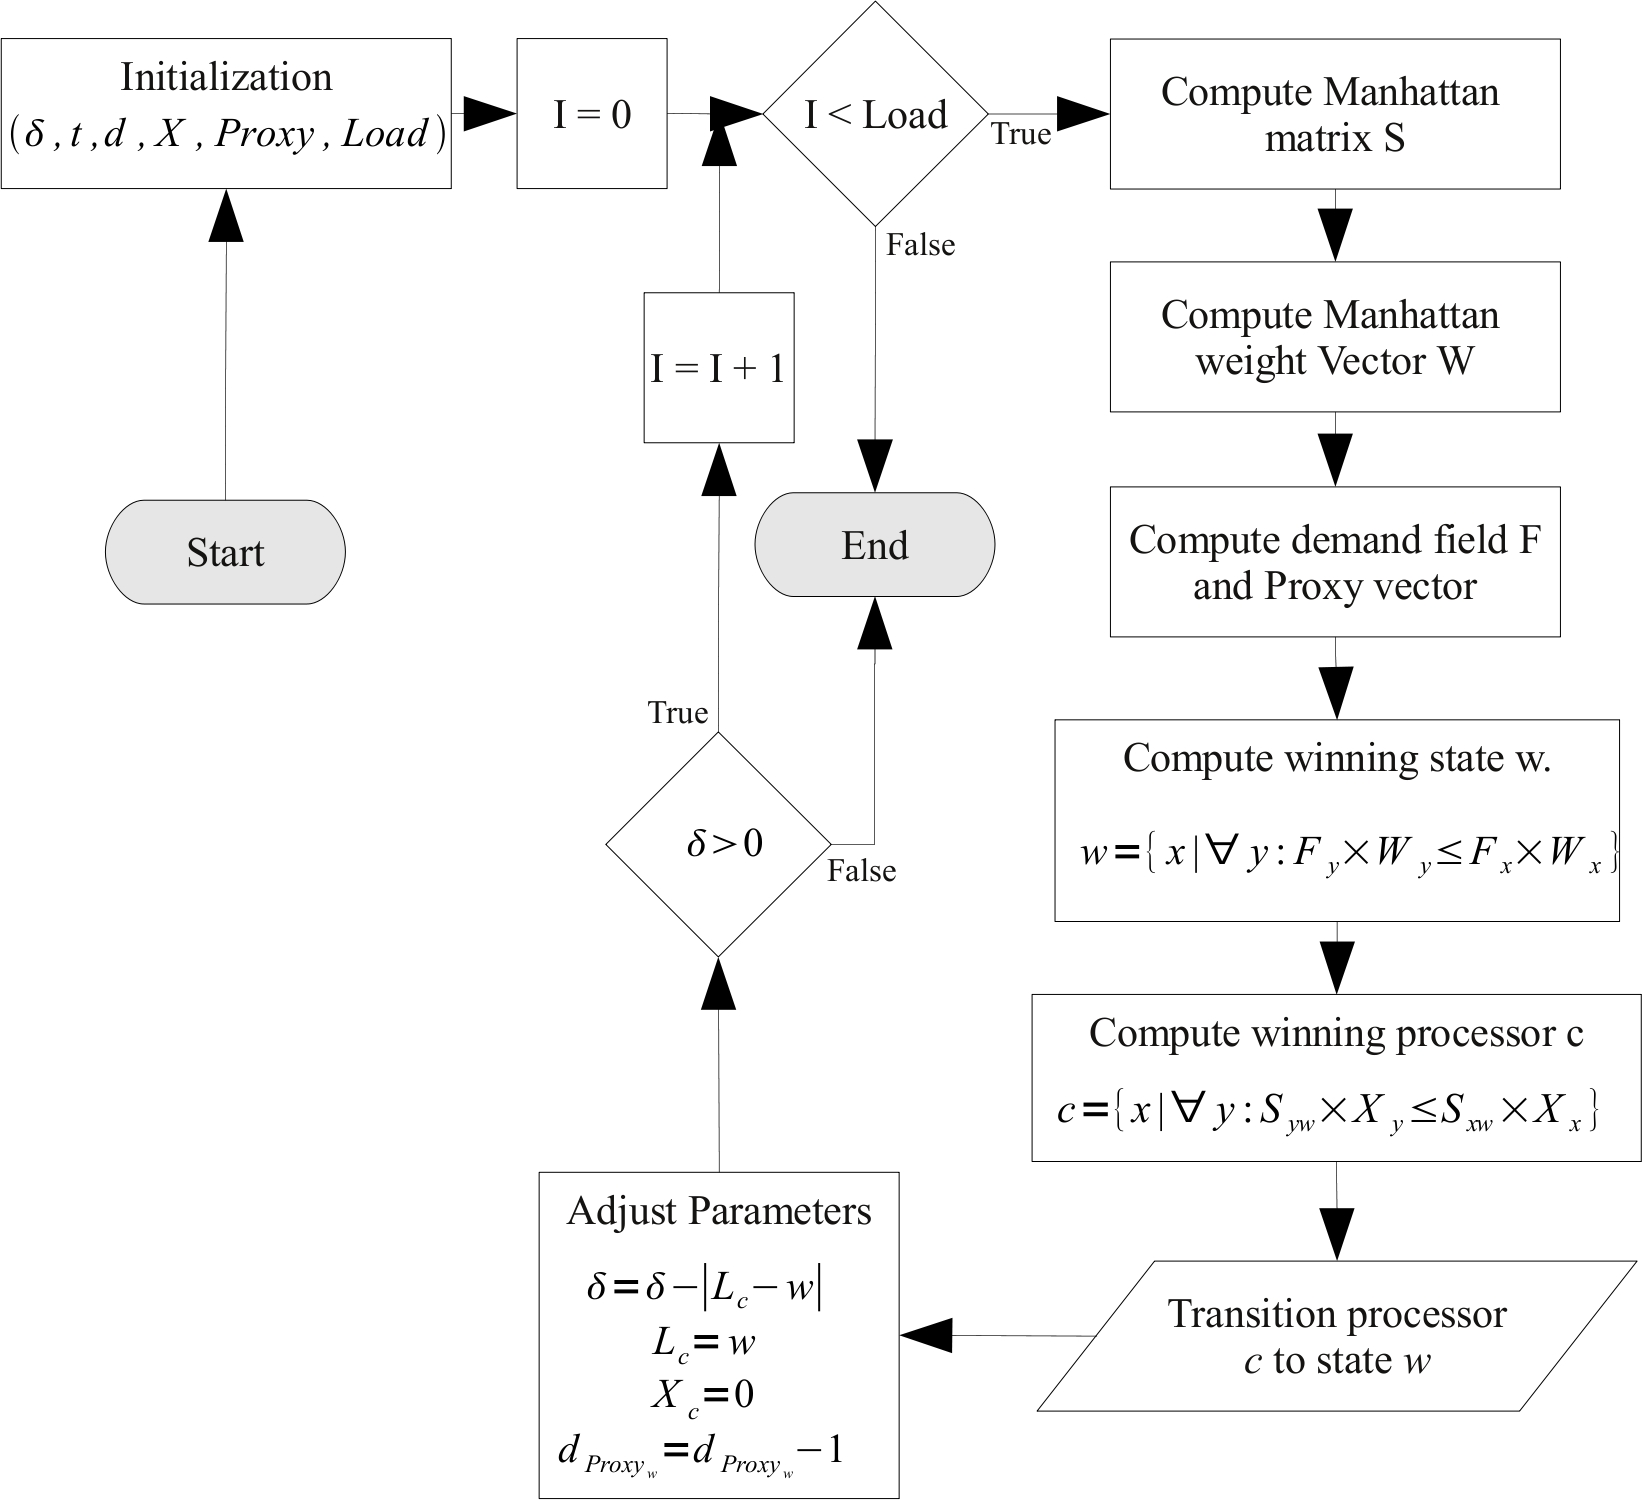
\includegraphics[height=4in]{figures/Mutation_algo.jpg}
    \caption{Mutation algorithm}
    \label{fig:mutation_algo}
  \end{center}
\end{figure}

%%%%%%%%%%%%%%%%%%%%%%%%%%%%%%%%%%%%%%%%%%%%%%%%%%%%%%%%%%%%%%%%%%%%%%%%%%%%%%%
\subsection{Initialization}~\label{sec:mut_init}
%%%%%%%%%%%%%%%%%%%%%%%%%%%%%%%%%%%%%%%%%%%%%%%%%%%%%%%%%%%%%%%%%%%%%%%%%%%%%%%

In order to effectively provide only the needed number of processors, the mutator
queries the operating system for the total number of tasks in the ready state $T$. 
From which, the Load of the system in terms of number of processors required is computed 
as shown below in Equation~\eqref{eq:projected_load},
\begin{equation}
    Load = \left\{
     \begin{array}{lr}
       T & : T \leq N\\
       N & : T > N
     \end{array}
   \right.
\label{eq:projected_load}
\end{equation}
where $T$ is the total number of tasks in the ready state in a multi-processor system with \textit{N} online processors.
Using an estimated load based on idle times
of processors was found to be unfruitful as it can be non-representative of the actual 
computing capacity demanded by the number of active tasks. This can be emphasized in situations where multiple
tasks could be queued on a single processor.

The Performance Directed Scheduler as described in Chapter~\ref{chap:pds} maintains
the demand for each state in the demand vector \textbf{D}. The contents of this vector
cannot be directly consumed as their values pose no direct description of the demand 
of individual performance states. As a direct consequence, vector \textbf{d} is computed based 
on the projected load of the system and the demand vector \textbf{D} shown below in Equation~\eqref{eq:processor_demand},
\begin{equation}
    d_{i} = \frac{D_{i} \times Load}{\displaystyle\sum_{j=0}^{M-1} {D_{j}}}
\label{eq:processor_demand}
\end{equation}
where $D_i$ is the total number of times performance state $P_i$ was requested by the performance directed scheduler in 
the previous mutation interval while the total load of the system was estimated to be \textit{load}. The vector \textbf{d}
is also reffered to as the processor demand as each element $d_i$ is the total number of processors demanded by the 
performance directed scheduler in state $P_i$. 

$Z_P$ the present or current power number of the multi-processor system is computed as shown below in Equation~\eqref{eq:Z_P},
\begin{equation}
    Z_{P} = \displaystyle\sum_{i=0}^{N-1} {L_{i}} 
\label{eq:Z_P}
\end{equation}
where \textit{N} is the total number of online processors and \textbf{L} is the current layout of the system. Thus $Z_P$ 
is an integer value proportional to the total power drawn by the multi-processor system. $Z_R$, the required power number  is computed based on the 
processor demand \textbf{d} as shown below in Equation~\eqref{eq:Z_R},
\begin{equation}
    Z_{R} = \displaystyle\sum_{i=0}^{M-1} {i \times d_{i}} 
\label{eq:Z_R}
\end{equation}
where, each processor is capable of \textit{M} performance states and $d_i$ being the total number of processors demanded
by performance state $P_i$. Thus $Z_R$ is proportional to the power drawn by the multi-processor system when the processors
are transitioned in such a way as to satisfy the performance directed scheduler to optimally assign current tasks. 

Based on $Z_{P}$ and $Z_{R}$, the transition direction, \textit{t}, a tri-state value describing the nature of 
mutation required is computed as shown below in Equation~\eqref{eq:transition_dir}. 
\begin{equation}
    t = \left\{
     \begin{array}{lr}
       1 & : Z_{R} > Z_{P}\\
       0 & : Z_{R} = Z_{P} \\
       -1 & : Z_{R} < Z_{P}
     \end{array}
   \right.
\label{eq:transition_dir}
\end{equation}
A transition direction of $t = +1$ implies that the scheduler requires higher performance from
the multi-processor, while a transition direction of $t = -1$ implies the exact opposite; an indication
to conserve power by reducing the performance states of the multi-processor. A transition direction equal to zero
implies stability and and mutations must be avoided if possible. 

Before starting the iterations, the poison vector \textbf{X} of length \textit{N} is initialized to all ones, where
each element corresponds to a processor. Each element of the poison vector is a binary element with a value of 0 
implying that the processor has been allocated a performance state and must not be re-transitioned, The initialization
of the poison vector is described below in Equation~\eqref{eq:poison_init} for a multi-processor system with \textit{N} processors.
\begin{equation}
    \forall i : 0 \geq i < N; X_{i} = 1 
\label{eq:poison_init}
\end{equation}
The iteration delta constraint $\delta$ is initialized to $\Delta$  ($\delta = \Delta$). 

%%%%%%%%%%%%%%%%%%%%%%%%%%%%%%%%%%%%%%%%%%%%%%%%%%%%%%%%%%%%%%%%%%%%%%%%%%%%%%%
\subsection{The Manhattan matrix}~\label{sec:delta_matrix}
%%%%%%%%%%%%%%%%%%%%%%%%%%%%%%%%%%%%%%%%%%%%%%%%%%%%%%%%%%%%%%%%%%%%%%%%%%%%%%%

The Manhattan matrix \textbf{S} of dimension $N \times M$, can be viewed as a probability matrix where each element
$S_{ij}$ indicates the probability that processor \textit{i} can be transitioned to
performance state \textit{j} for a system with \textit{N} processors each 
capable of \textit{M} transition states. The conception of this matrix was achieved by viewing
a probability density function for each processor and was soon modified due to the lack of floating point operations in kernel space 
(Even though possible, the kernel address space does not save the floating point 
context and makes it's use dangerous as the kernel is fully preempt-able).

The Manhattan matrix ($N \times T$) is computed as shown below (Equation~\eqref{eq:delta_mat}),
\begin{equation}
    \forall i,j \in \mathbb{N} : i < N, j < M; S_{ij} = \left\{
     \begin{array}{lcr}
       0 & : & j < (L_{i} - \delta) \\
       \frac{M}{2} \times (t^{2} - t + 2) + j - L_{i} & : & (L_{i} - \delta) \leq j < L_{i} \\
       2M & : & j = L_{i}\\
       \frac{M}{2} \times (t^{2} + t + 2) - j + L_{i} & : & L_{i} < j \leq (L_{i} + \delta) \\
       0 & : & j > (L_{i} + \delta)
     \end{array}
   \right.
\label{eq:delta_mat}
\end{equation}
where, $L_i$ is the current performance state of processor \textit{i} in a multi-processor enviornment 
with a total of \textit{N} processors each processor capable of \textit{M} performance states 
and the transition direction \textit{t} estimated to be either $-1$, $0$ or $+1$. 

Each row in the Manhattan matrix corresponds to an on-line processor core while each column corresponds to a performance state
in increasing order. Thus $S_{23}$ describes the weight of processor $C_2$ transitioning to the performance state $P_3$. 
For example, consider a hypothetical multiprocessor with a total of 4 processors ($N = 4$) each capable of
5 performance states ($M = 5$) with the current layout \textbf{L} = [0,1,2,3], implying that processors $C_0$, $C_1$, $C_2$ and $C_3$
are in performance states $P_0$, $P_1$, $P_2$ and $P_4$ respectively. 

Based on the processor demand, if the transition direction $t = 1$, implying higher required performance
out of the multi-processor system, and the iteration delta constraint $\delta = 2$, then the Manhattan matrix \textbf{S} 
is shown below (Equation~\eqref{eq:ex_dmuth}).
\begin{equation}
    S^{t = +1} = \left[
     \begin{array}{ccccc}
       10 & 9 & 8 & 0 & 0 \\
       4 & 10 & 9 & 8 & 0 \\
       3 & 4 & 10 & 9 & 8 \\
       0 & 3 & 4 & 10 & 9
     \end{array}
   \right]
\label{eq:ex_dmuth}
\end{equation}
The following can be observed about this matrix (Equation~\eqref{eq:ex_dmuth}):
\begin{enumerate}
\item For each row, \textit{i}, the highest weight of $2M$ (10), is assigned to the element $S_{ij}$ when $j = L_i$. Thus, as $L_0 = 0$, the element $S_{00} = 10$.
\item For each row, \textit{i}, elements $S_{ij}$ are assigned a value of 0, when they are more that $\delta$ elements away ($|j - L_i| > \delta$). Thus elements $S_{03}$ and $S_{04}$
are assigned a value of 0.
\item For each row, \textit{i}, and column $L_i < j \leq (L_i + \delta)$, integer values are assigned to $S_{ij}$ such that they are in decreasing order starting from $2M-1$ (9).
Thus $S_{01}$, $S_{02}$ are given values 9 and 8 respectively. 
\item For each row, \textit{i}, and column $(L_i - \delta) \leq j < L_i$, integer values are assigned to $S_{ij}$ such that they are in decreasing order starting from $M-1$ (4).
Thus $S_{21}$ and $S_{20}$ are given values 4 and 3 respectively.
\end{enumerate}
This construction for a transition direction $t = 1$ favors transitions towards higher performance states. 

For the same example of $N = 4$, $M = 5$, $\delta = 2$ and finally $L = [0,1,2,3]$, the Manhattan matrix \textbf{S} for a transition direction $t = 0$ is shown below (Equation~\eqref{eq:ex_dmut0}).
\begin{equation}
    S^{t = 0} = \left[
     \begin{array}{ccccc}
       10 & 4 & 3 & 0 & 0 \\
       4 & 10 & 4 & 3 & 0 \\
       3 & 4 & 10 & 4 & 3 \\
       0 & 3 & 4 & 10 & 4
     \end{array}
   \right]
\label{eq:ex_dmut0}
\end{equation}
The following can be observed about this matrix (Equation~\eqref{eq:ex_dmut0}):
\begin{enumerate}
\item For each row, \textit{i}, the highest weight of $2M$ (10), is assigned to the element $S_{ij}$ when $j = L_i$. Thus, as $L_0 = 0$, the element $S_{00} = 2 \times 5$.
\item For each row, \textit{i}, elements $S_{ij}$ are assigned a value of 0, when they are more that $\delta$ elements away ($|j - L_i| > \delta$). Thus elements $S_{03}$ and $S_{04}$
are assigned a value of 0.
\item For each row, \textit{i}, and column $L_i < j \leq (L_i + \delta)$, integer values are assigned to $S_{ij}$ such that they are in decreasing order starting from $M-1$ (4).
Thus $S_{01}$, $S_{02}$ are given values 4 and 3 respectively. 
\item For each row, \textit{i}, and column $(L_i - \delta) \leq j < L_i$, integer values are assigned to $S_{ij}$ such that they are in decreasing order starting from $M-1$ (4).
Thus $S_{21}$ and $S_{20}$ are given values 4 and 3 respectively.
\end{enumerate}
This construction for a transition direction $t = 0$ favors transitions in either direction equally. 

Finally, the Manhattan matrix for a transition direction $t = -1$ is shown below (Equation~\eqref{eq:ex_dmutl}).
\begin{equation}
    S^{t = -1} = \left[
     \begin{array}{ccccc}
       10 & 4 & 3 & 0 & 0 \\
       9 & 10 & 4 & 3 & 0 \\
       8 & 9 & 10 & 4 & 3 \\
       0 & 8 & 9 & 10 & 4
     \end{array}
   \right]
\label{eq:ex_dmutl}
\end{equation}
The following can be observed about this matrix (Equation~\eqref{eq:ex_dmutl}):
\begin{enumerate}
\item For each row, \textit{i}, the highest weight of $2M$ (10), is assigned to the element $S_{ij}$ when $j = L_i$. Thus, as $L_0 = 0$, the element $S_{00} = 2 \times 5$.
\item For each row, \textit{i}, elements $S_{ij}$ are assigned a value of 0, when they are more that $\delta$ elements away ($|j - L_i| > \delta$). Thus elements $S_{03}$ and $S_{04}$
are assigned a value of 0.
\item For each row, \textit{i}, and column $L_i < j \leq (L_i + \delta)$, integer values are assigned to $S_{ij}$ such that they are in decreasing order starting from $M-1$ (4).
Thus $S_{01}$, $S_{02}$ are given values 4 and 3 respectively. 
\item For each row, \textit{i}, and column $(L_i - \delta) \leq j < L_i$, integer values are assigned to $S_{ij}$ such that they are in decreasing order starting from $2M-1$ (9).
Thus $S_{21}$ and $S_{20}$ are given values 9 and 8 respectively.
\end{enumerate}
This construction for a transition direction $t = -1$ favors transitions which reduce the performance state of each processor. 


%%%%%%%%%%%%%%%%%%%%%%%%%%%%%%%%%%%%%%%%%%%%%%%%%%%%%%%%%%%%%%%%%%%%%%%%%%%%%%%
\subsection{The Manhattan weight vector}~\label{sec:weight}
%%%%%%%%%%%%%%%%%%%%%%%%%%%%%%%%%%%%%%%%%%%%%%%%%%%%%%%%%%%%%%%%%%%%%%%%%%%%%%%

The Manhattan weight vector $W$ is constructed as shown below (Equation~\ref{eq:state_weight}),
\begin{equation}
    \forall j \in \mathbb{N} : j < M; W_j = \displaystyle\sum_{i=0}^{N-1} {S_{ij}}
\label{eq:state_weight}
\end{equation}
where \textit{N} is the total number of processors and \textit{M} is the total number of
performance states each processors is capable of.
The Manhattan weight vector is achieved by summing along each column 
of the Manhattan matrix and hence providing an insight of the locality of each state. A higher value of $W_i$ 
indicates a higher probability that there exists active processors in or around
performance state \textit{i}, while a null value, $W_i = 0$ indicates that the performance state \textit{i}
can never be achieved under the current delta constraint. 


%%%%%%%%%%%%%%%%%%%%%%%%%%%%%%%%%%%%%%%%%%%%%%%%%%%%%%%%%%%%%%%%%%%%%%%%%%%%%%%
\subsection{Cooperative demand distribution: The demand field}~\label{sec:field}
%%%%%%%%%%%%%%%%%%%%%%%%%%%%%%%%%%%%%%%%%%%%%%%%%%%%%%%%%%%%%%%%%%%%%%%%%%%%%%%

With lower values of $\Delta$, there is a possibility that a state \textit{i},
could be requested with a high demand $d_i$ but due to the current layout and 
delta constraint, have a Manhattan weight $W_i = 0$, implying that a processor 
in performance state \textit{i} can never be provided.
Thus a method was developed in transforming the demand vector \textbf{d}
in such a way that such null performance states cooperatively give up their demand
to the performance state closest to them which has a possibility of being selected. 
This procedure is described in Algorithm~\ref{fig:field}.


\begin{algorithm}[h!]
 \SetLine
 \KwIn{Demand vector \textbf{d}, Manhattan weight vector \textbf{W}}
 \KwOut{Demand field \textbf{F}, Proxy vector \textbf{Proxy}}
 \ForEach{Performance state $i$}{
     $Proxy_i = i$ \;
     $F_i = d_i$ \;
 }
 \ForEach{Performance state $i$}{
   \If{$W_i = 0$ and $d_i > 0$}{
      \If{$t = 1$}{
        $f = max \{ x : x \in N \wedge x < i \wedge W_x > 0 \}$ \;
      }
      \If{$t = -1$}{
        $f = min \{x : x \in N \wedge x > i \wedge W_x > 0 \}$ \;
      }
      \If{$t = 0$}{
        $f = x : x \in N \wedge x \approx i \wedge W_x > 0$ \;
         f is closest to i such that weight $W_f > 0$.
      }
      $F_f = F_f + F_i$ \;
      $F_i = 0$ \;
      $Proxy_f = i$ \;
    }
 }
\caption{Demand field computation}
\label{fig:field}
\end{algorithm}

The demand field \textbf{F} is essentially a replicate of \textbf{d}, and differs under
circumstances when for a particular performance state \textit{i}, $W_i = 0$ and $d_i > 0$,
then its demand is distributed to a friend \textit{f} which varies based on the transition
direction t. If transition direction $t = 1$, then the demand is given to the state \textit{f} closest and lesser than
\textit{i} with $W_f > 0$. If the transition direction $t = -1$ then a friend is searched in 
the opposite direction with $W_f > 0$. Finally when $t = 0$, the closest state \textit{f} to \textit{i} with $W_f > 0$ is chosen as the 
friend. Once the friend state \textit{f} is computed, all the demand $d_i$ is transferred \textit{f}.
In order to track contributions from others, a vector \textbf{Proxy} is maintained indicating 
the source of the demand. Under normal circumstances, $Proxy_i = i$. 

%%%%%%%%%%%%%%%%%%%%%%%%%%%%%%%%%%%%%%%%%%%%%%%%%%%%%%%%%%%%%%%%%%%%%%%%%%%%%%%
\subsection{Greedy performance state selection}~\label{sec:winner_state}
%%%%%%%%%%%%%%%%%%%%%%%%%%%%%%%%%%%%%%%%%%%%%%%%%%%%%%%%%%%%%%%%%%%%%%%%%%%%%%%

Once \textbf{W} and \textbf{F} are computed, performance state \textit{w} is selected
as the winning state when the value of the product $W_w \times F_w$ is the maximum 
for all states \textit{i} and hence reacting to demand and maintaining locality. 
The procedure is mathematically depicted below (Equation~\eqref{eq:winning_state}),
\begin{equation}
    w = {x | \forall y, y \in \mathbb{N} \wedge 0 \leq y < M : W_y \times F_y \leq W_x \times F_x}
\label{eq:winning_state}
\end{equation}
where, \textit{N} is the total number of processors and \textit{M} is the number of
performance states each processor is capable of.

%%%%%%%%%%%%%%%%%%%%%%%%%%%%%%%%%%%%%%%%%%%%%%%%%%%%%%%%%%%%%%%%%%%%%%%%%%%%%%%
\subsection{Greedy processor selection and transition}~\label{sec:winner_proc}
%%%%%%%%%%%%%%%%%%%%%%%%%%%%%%%%%%%%%%%%%%%%%%%%%%%%%%%%%%%%%%%%%%%%%%%%%%%%%%%

With the winning performance state selected, the processor to be transitioned
is determined by the row \textit{c} in the Manhattan matrix whose value $S_{cw} \times X_c$ 
is maximum and shown below (Equation~\ref{eq:winning_proc}). 
\begin{equation}
    c = {x | \forall y, y \in \mathbb{N} \wedge 0 \leq y < N : S_{yw} \times X_y \leq S_{xw} \times X_x}
\label{eq:winning_proc}
\end{equation}

Once the selection is made, processor \textit{c} is transitioned to performance state
\textit{w} by invoking the seeker cpufreq governor described in Section~\ref{sec:cpufreq}.


%%%%%%%%%%%%%%%%%%%%%%%%%%%%%%%%%%%%%%%%%%%%%%%%%%%%%%%%%%%%%%%%%%%%%%%%%%%%%%%
\subsection{Parameter change and termination conditions}~\label{sec:param_adjust}
%%%%%%%%%%%%%%%%%%%%%%%%%%%%%%%%%%%%%%%%%%%%%%%%%%%%%%%%%%%%%%%%%%%%%%%%%%%%%%%

At the end of every iteration, the parameters $\delta$, $L_c$ and $d_p$ are updated
to represent the transition. First as a transition was previously performed, the iteration delta constraint
must reduce by an equal order as shown below (Equation~\eqref{eq:update_delta}).
\begin{equation}
    \delta = \delta - |L_{c} - w| 
\label{eq:update_delta}
\end{equation}
Second, as processor \textit{c} is no longer in performance state $L_c$, it is updated to
it's new value \textit{w} as shown below (Equation~\eqref{eq:update_L}) 
\begin{equation}
    L_{c} = w 
\label{eq:update_L}
\end{equation}
Third, as a processor is assigned to performance state \textit{w},
the corresponding demand can be reduced as shown below (Equation~\eqref{eq:update_d}).
\begin{equation}
    d_{Proxy_w} = d_{Proxy_w} - 1 
\label{eq:update_d}
\end{equation}
Note that, due to the distortion introduced by the cooperative demand distribution, $d_{Proxy_w}$ is updated
instead of $d_w$. 
Lastly, the poison vector's position for processor
\textit{c} is set to zero and hence disabling processor \textit{c} in participating in a future transition as shown
below (Equation~\eqref{eq:update_X}).
\begin{equation}
    X_c = 0
\label{eq:update_X}
\end{equation}

This concludes a single iteration of the greedy direction based algorithm and is repeated for \textit{Load} iterations
as long as the iteration delta constraint $\delta > 0$. The upper bound on the number of iterations is obviously \textit{Load} 
and ensures early termination of the iterative algorithm when unnecessary.




%%%%%%%%%%%%%%%%%%%%%%%%%%%%%%%%%%%%%%%%%%%%%%%%%%%%%%%%%%%%%%%%%%%%%%%%%%%%%%%
\chapter{Experimental setup and results}~\label{chap:results}
%%%%%%%%%%%%%%%%%%%%%%%%%%%%%%%%%%%%%%%%%%%%%%%%%%%%%%%%%%%%%%%%%%%%%%%%%%%%%%%

A Linux kernel module as shown in Figure~\ref{fig:entire_seeker} was developed incorporating the ideas 
discussed in chapters \ref{chap:pds} and \ref{chap:delta}. 
The scheduling routines in the Linux kernel (To be specific, \textit{schedule} and \textit{\_\_switch\_to})
were extended using kprobes \cite{kprobes} to add the performance directed scheduling features.
The choice to use kprobes \cite{kprobes} a feature essentially used for debugging and instrumentation
from the context of a kernel module pose two possible 
problems. One, kprobes by themselves introduce unnecessary code paths and interrupts causing some
if not significant overhead (Less than 3\%). Secondly, certain functions relating to migration are not exported
to kernel modules and hence indirect and suboptimal procedures were chosen to get the necessary 
functionality. In spite of these disadvantages, having the project as a kernel module accelerated 
the development process. 

For a system with \textit{M} total performance states and \textit{N} total processors, $\Delta$ can 
at most take a value of $N \times (M-1)$. Experiments were carried on a quad-core AMD Opteron (Barcelona),
and a patched version of the Linux 2.6.28 kernel. The logging interface as shown in Figure~\ref{fig:entire_seeker},
collects task specific and system wide statistics which enable in studying the behavior of both the performance
directed scheduler and the delta constrained mutator. The statistics collected by the logging system aided in 
the computation of the total energy consumption of each processor for each run workload. In order to measure 
percentage slowdown, the six workloads mentioned in Appendix~\ref{app:benchmark}, were run with full clock speed
and recording their cumulative execution time. In order to estimate power and energy consumption, the power 
values mentioned in \cite{AMDPow} (Provided in Appendix~\ref{app:opteron} for convenience) were utilized 
to compute the average power and energy consumption. Appendix~\ref{app:mutation_timeline} displays the 
adaptation time line graph showcasing each of the two schedulers along with the delta constrained mutator.

The system call interface allows an application runtime (or an application) to provide hints to the scheduler
on the performance state demanded and allows compiler and runtime power optimizing frameworks to interact with the underlying
power optimizer to create a more robust system. The discussion of the system call interface is beyond the scope 
of this text and will not be further discussed, but shown only as an example of possible extensions to the 
discussed power management system.

\begin{figure}[h!]
  \begin{center}
%    \resizebox{\columnwidth}{!}{
    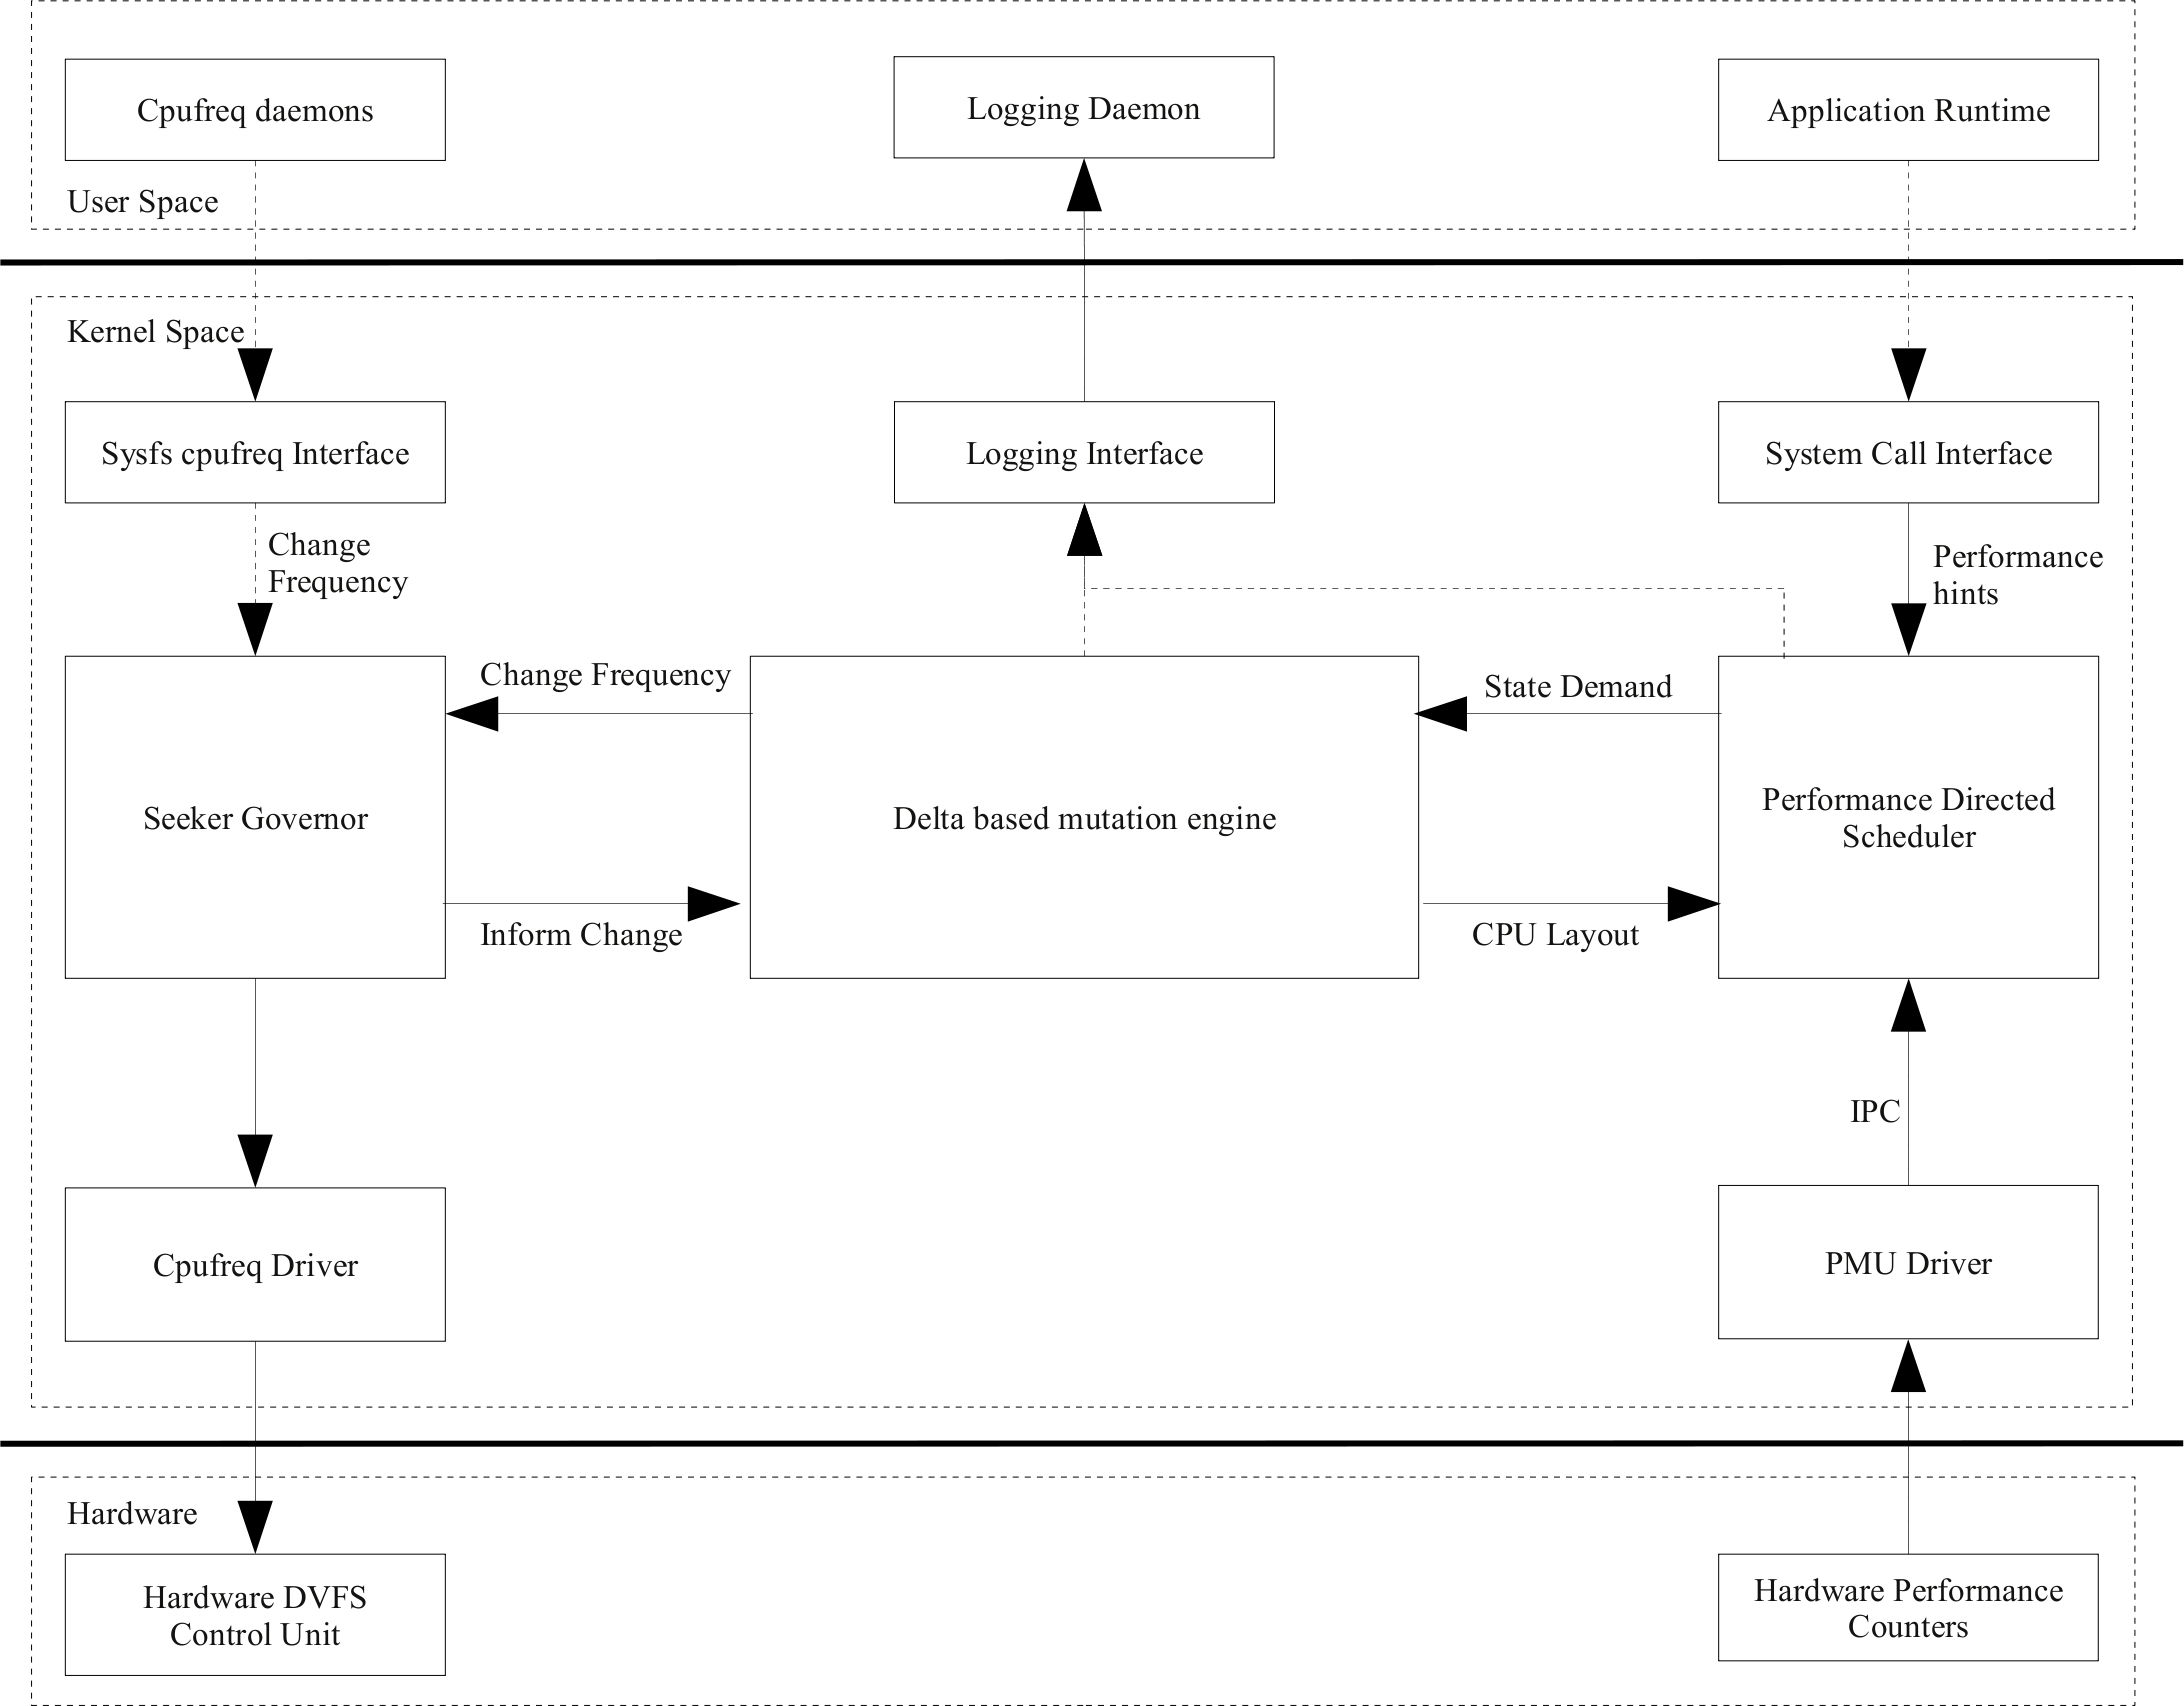
\includegraphics[height=4in]{figures/seeker.jpg}%}
    \caption{The Seeker infrastructure}
    \label{fig:entire_seeker}
  \end{center}
\end{figure}

%%%%%%%%%%%%%%%%%%%%%%%%%%%%%%%%%%%%%%%%%%%%%%%%%%%%%%%%%%%%%%%%%%%%%%
% START REAL GRAPHS
%%%%%%%%%%%%%%%%%%%%%%%%%%%%%%%%%%%%%%%%%%%%%%%%%%%%%%%%%%%%%%%%%%%%%%
%%%%%%%%%%%%%%%%%%%%%%%%%%%%%%%%%%%%%%%%%%%%%%%%%%%%%%%%%%%%%%%%%%%%%%%%%%%%%%%
\section{Trends along delta and interval}~\label{sec:trends}
%%%%%%%%%%%%%%%%%%%%%%%%%%%%%%%%%%%%%%%%%%%%%%%%%%%%%%%%%%%%%%%%%%%%%%%%%%%%%%%

Two parameters namely the delta constraint ($\Delta$) and the mutation interval 
were introduced in Chapter~\ref{chap:delta}. In order to further study the system
it is important to define the variation of two important effects,
namely, slowdown and power savings, as a function of these parameters. In order
to accomplish the study, a fully factorial experiment was conducted varying delta 
from 1 to 16 and the interval from 125ms to 1000ms. All the six workloads in 
Table~\ref{tab:spec_groups} in Appendix~\ref{app:benchmark} were run in each 
experiment. Slowdown for each experiment was computed by comparing the execution time of each workload 
to that when run on a multi-processor system with all processors executing with the maximum frequency.


Figure~\ref{fig:slowdown_trends} show the trends
observed with respect to slowdown for the ladder and select schedulers. An unnaturally 
high slowdown can be observed for small values of delta ($\Delta$) and can be attributed
to the plasticity in adaptation. The interval of mutation has little significance towards slowdown
for delta values higher than 3 but when lowered beyond 3, the mutation interval begins to play a vital 
role in differentiating the experiments based on slowdown. It can be observed that at lower values
of delta, reducing the mutation interval has an effect of decreasing the slowdown and effectively 
reducing the performance lost. Comparing Figure~\ref{fig:slowdown_trends_ladder} 
with \ref{fig:slowdown_trends_select} shows that the select scheduling system is largely affected
by lower values of delta than the ladder scheduling system. At $\Delta = 1$, the select scheduling
system exhibits at least 5\% increased in slowdown when compared to the ladder scheduling system but 
both rapidly falls to the plateau close to 16\% beyond a delta constraint of 4. 

\begin{figure}[h!]
\centering
%  \begin{center}
  \subfigure[Ladder scheduler]{
    %\resizebox{\columnwidth}{!}{
    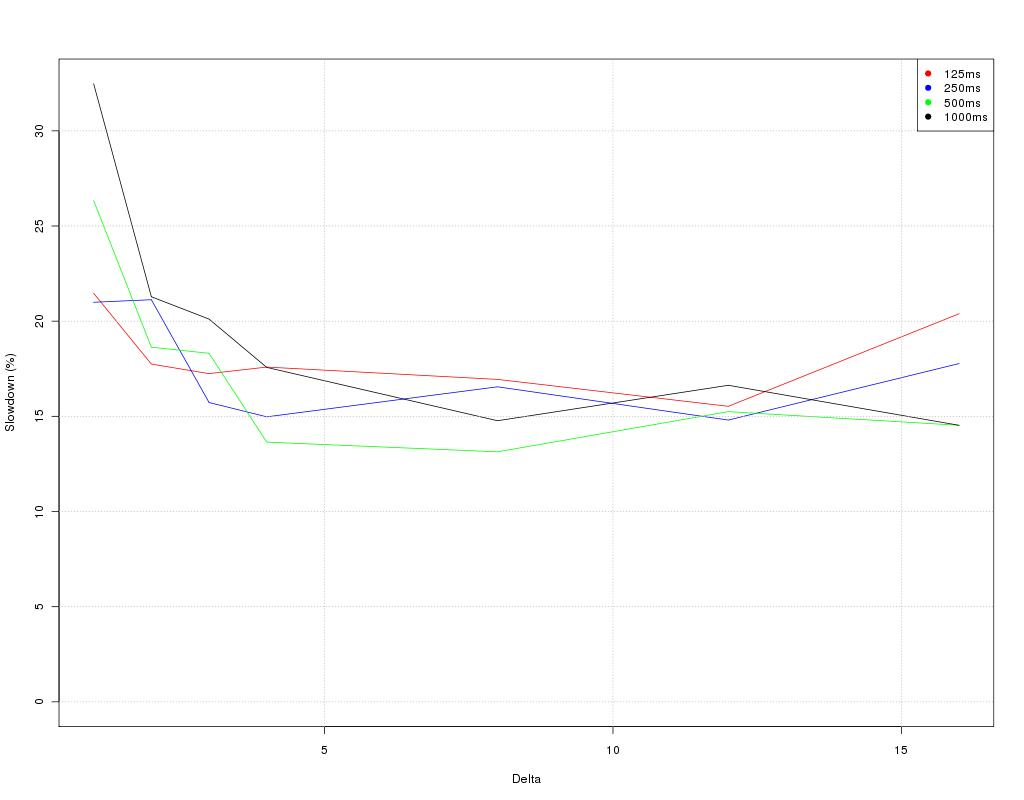
\includegraphics[height=2.5in]{figures/trends_slowdown_ladder.jpg}%}
%\caption{Variation of slowdown with delta and interval with the ladder scheduler}
    \label{fig:slowdown_trends_ladder}
  }
%  \end{center}
%\end{figure}

%\begin{figure}[h!]
%  \begin{center}
    %\resizebox{\columnwidth}{!}{
   \subfigure[Select scheduler]{
    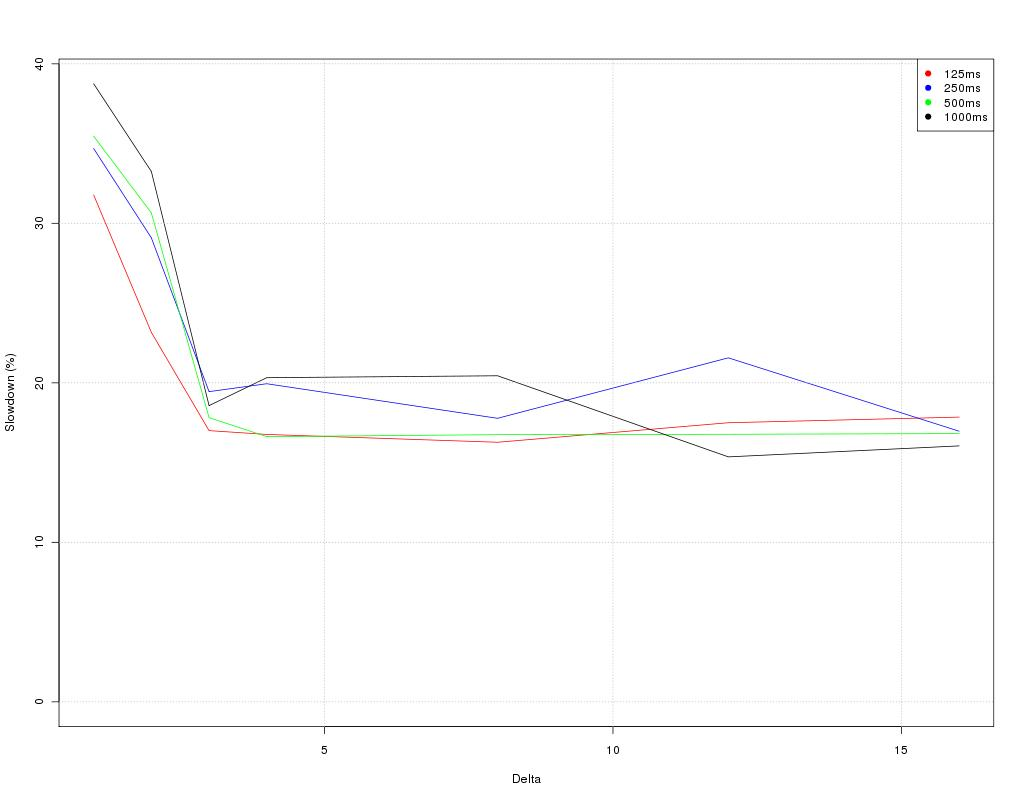
\includegraphics[height=2.5in]{figures/trends_slowdown_select.jpg}%}
%    \caption{Variation of slowdown with delta and interval with the select scheduler}
    \label{fig:slowdown_trends_select}
  }
  \label{fig:slowdown_trends}
%  \end{center}
  \caption{Variation of slowdown with delta and interval for the ladder \subref{fig:slowdown_trends_ladder} and the select \subref{fig:slowdown_trends_select} scheduler}
\end{figure}

In order to study the power conservation, the logging interface was sampled to acquire
an execution sample's execution time and performance state (and in effect the power consumption
when compared to Table~\ref{tab:perf_power}). The average power consumption was computed 
by computing the energy consumption of each execution sample and in effect the overall 
energy consumption. The total energy consumption was divided by the total execution time
to arrive at the average power consumption. The percentage power savings is computed
by comparing the average power consumption to the maximum power consumption (at the highest
frequency) is 115.0W (Table~\ref{tab:perf_power}).

Figure~\ref{fig:pwr_trends} shows the variation of percentage power savings with varied value 
of delta ($\Delta$) and mutation interval. A trend similar to percentage slowdown is observed
for power savings: A high value of power savings for lower values of delta which drop sharply 
at the value of $\Delta = 3$. Even though high power savings are desirable, the effective 
slowdown accompanying this can be disadvantageous. A trend unique to power savings is the 
continued effect of mutation interval, whose decrease improves power savings marginally.
During the experimentation, mutation intervals lower than 100ms was observed to cause system
instabilities and frequent crashes and hence the study was performed only for values starting
from 125ms, even though can be attributed to the implementation, \cite{ImpactDVFS} warns 
system designers to avoid rapid DVFS transitions and hence must be avoided.


\begin{figure}[h!]
\centering
%  \begin{center}
    %\resizebox{\columnwidth}{!}{
  \subfigure[Ladder scheduler]{
    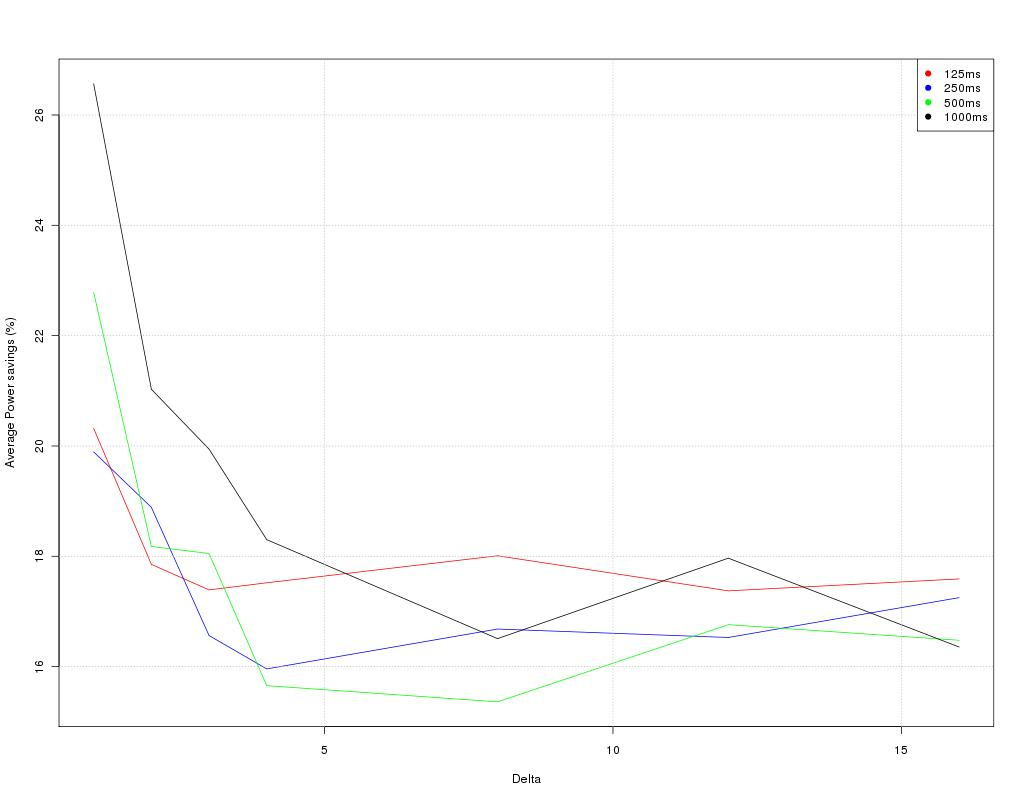
\includegraphics[height=2.5in]{figures/trends_avgpwr_ladder.jpg}%}
%    \caption{Variation of power savings with delta and interval with the ladder scheduler}
    \label{fig:pwr_trends_ladder}
  }
%  \end{center}
%\end{figure}

%\begin{figure}[h!]
%  \begin{center}
   \subfigure[Select scheduler]{
    %\resizebox{\columnwidth}{!}{
    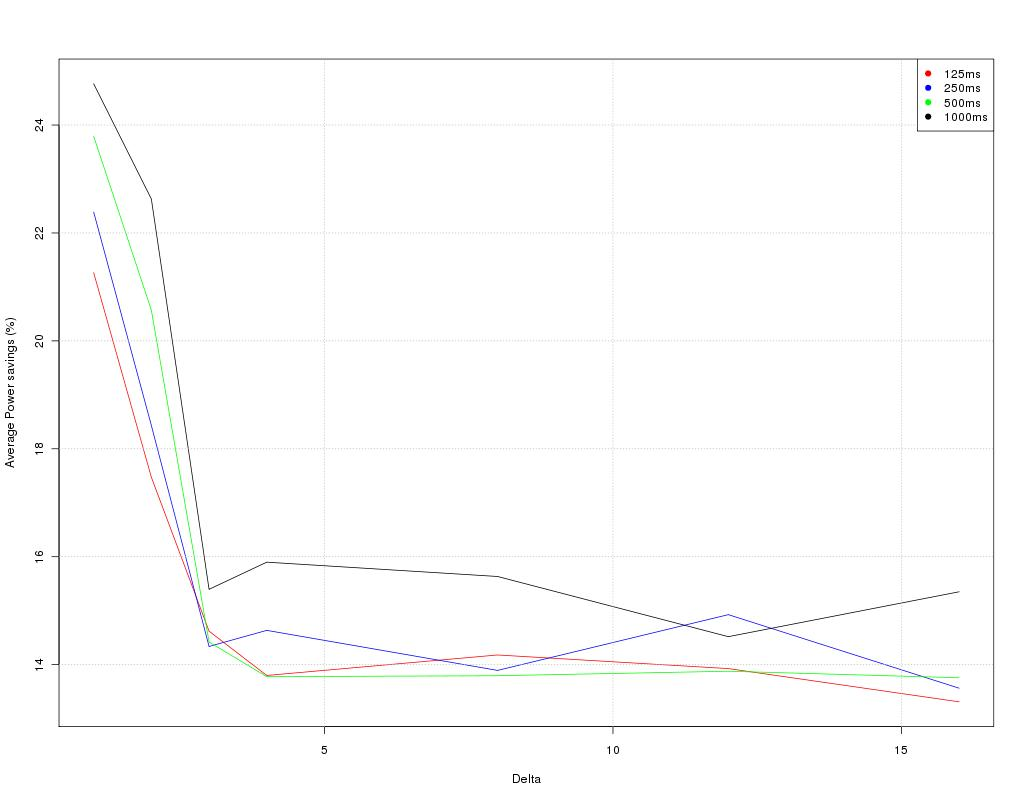
\includegraphics[height=2.5in]{figures/trends_avgpwr_select.jpg}%}
%    \caption{Variation of power savings with delta and interval with the select scheduler}
    \label{fig:pwr_trends_select}
  }
    \label{fig:pwr_trends}
    \caption{Variation of average power savings with delta and interval for the ladder (Subfigure~\subref{fig:pwr_trends_ladder}) and the select (Subfigure~\subref{fig:pwr_trends_select}) scheduler}
%  \end{center}
\end{figure}

Based on these observations, it can be concluded that a value of delta $\Delta = 4$ provides
the best among all the compromises and the interval can be changed based on the arrival rate
of jobs on the server or compute node. Having a very low mutation interval can hamper 
potential power savings for systems with a high mean time between execution workloads 
hence advising system designers to consider all these parameters before deploying the delta
constrained mutator.

%%%%%%%%%%%%%%%%%%%%%%%%%%%%%%%%%%%%%%%%%%%%%%%%%%%%%%%%%%%%%%%%%%%%%%%%%%%%%%%
\section{Effects of workload on power and performance}~\label{sec:wrk_trends}
%%%%%%%%%%%%%%%%%%%%%%%%%%%%%%%%%%%%%%%%%%%%%%%%%%%%%%%%%%%%%%%%%%%%%%%%%%%%%%%

Due to the adaptive nature of the power management mechanism and the high dependence
on the IPC characteristic of workloads, it can be hypothesized
that workloads with lower IPC (The \textit{Low} workload) should expect the maximum
power savings while, workloads with a large IPC (The \textit{High} workload) should
expect the minimum slowdown and power savings.
The power savings and slowdown box plots were drawing showcasing their characteristics and 
variation for each workload. It must be noted that the data from the experiments 
performed for the study presented in Section~\ref{sec:trends} were reused for the 
current analysis and was not pruned to the best values of delta and mutation interval. 
This study enables the study of the maximum impact of the variation of these parameters
(delta and mutation interval) for each workload. 

Figure~\ref{fig:workload_trends} shows the variation of percentage slowdown and power savings 
for each workload with both the scheduler systems. The \textit{High} workload 
suffers the minimum performance loss at a median close to 0\%. This is due to the fact 
that the adaptive scheduling system adapts to its high IPC characteristic and rapids 
provides it processors with the highest possible clock speed and hence explaining 
the insignificant slowdown. On the other hand, the \textit{Low} workload suffers a slowdown
of close to 17\% while providing an excess of 40\% power savings for the ladder scheduling
system. As the characteristic of the \textit{Low} workload is an average value of IPC below 0.5, 
the ladder system rapidly adapts to providing the workload the lowest clock speed and 
in turn conserving power. This displays the advantage of a workload based power optimizing 
system where the clock speed can be reduced by half its value and still certain workloads
can suffer at the most 20\% slowdown but providing up to 50\% in power savings. 

As the select scheduling system provides the \textit{Low} a higher clock speed than the 
ladder scheduling system (Observable in Appendix~\ref{app:mutation_timeline}, 
Figures~\ref{fig:wrk_low_ladder} and \ref{fig:wrk_low_select}), the power savings is 
noticeable lower. A high variance of slowdown can be observed for the \textit{High} 
workload running on the select scheduler indicating the cause of the additional slowdown
suffered by the select scheduling system when compared to the ladder system.

\begin{figure}[h!]
\centering
%  \begin{center}
  \subfigure[Ladder scheduler]{
    %\resizebox{\columnwidth}{!}{
    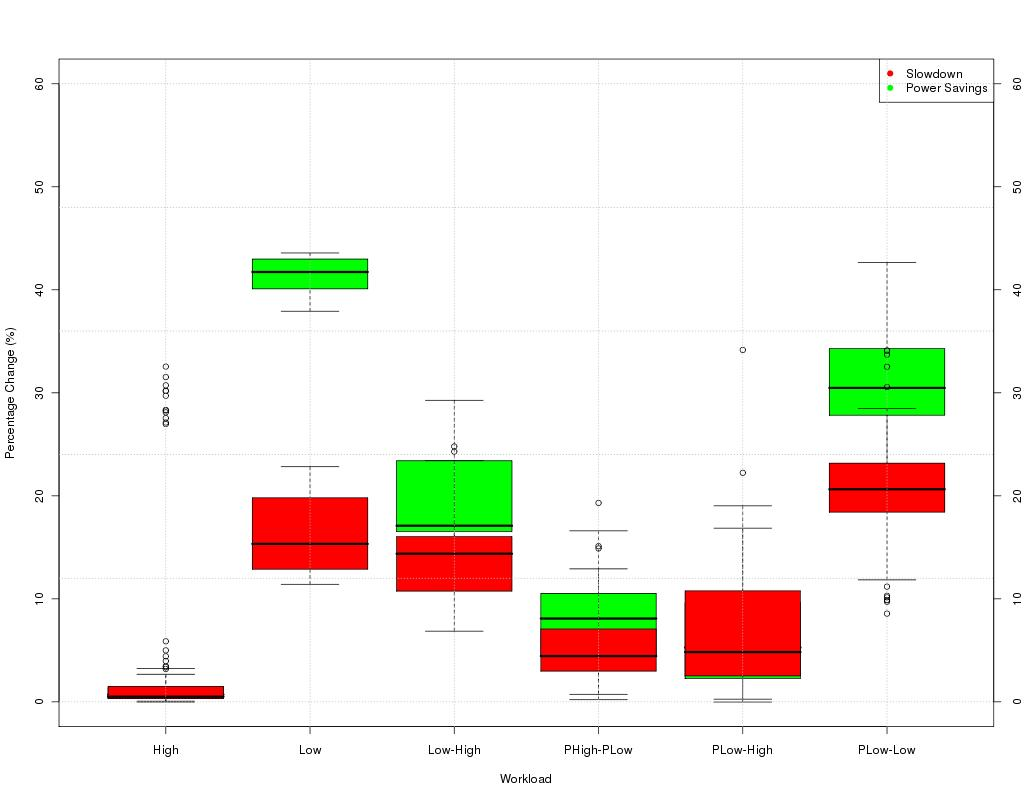
\includegraphics[height=2.5in]{figures/trends_workload_ladder.jpg}%}
%    \caption{Variation of slowdown and power savings for each workload with the ladder scheduler}
    \label{fig:workload_trends_ladder}
%  \end{center}
  }
%\end{figure}
%\begin{figure}[h!]
%  \begin{center}
   \subfigure[Select scheduler]{
    %\resizebox{\columnwidth}{!}{
    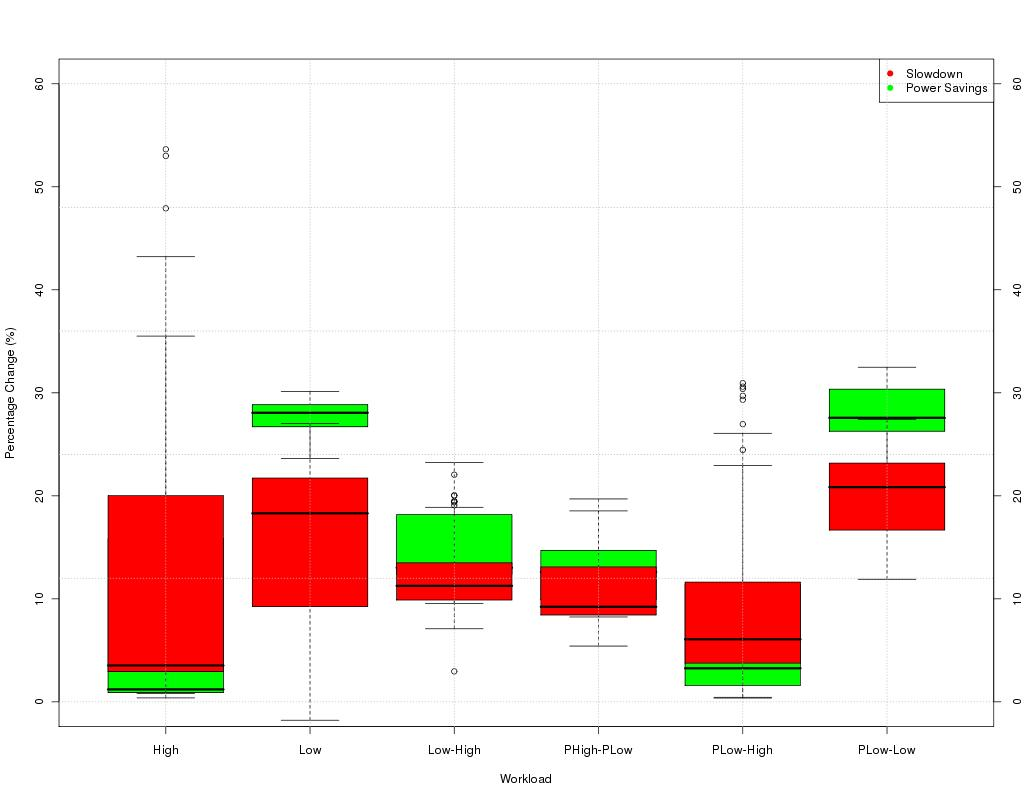
\includegraphics[height=2.5in]{figures/trends_workload_select.jpg}%}
%    \caption{Variation of slowdown and power savings for each workload with the select scheduler}
    \label{fig:workload_trends_select}
  }
%  \end{center}
\label{fig:workload_trends}
\caption{Variation of slowdown and power savings for each workload for the ladder (Subfigure~\subref{fig:workload_trends_ladder}) and the select (Subfigure~\subref{fig:workload_trends_select}) scheduler}
\end{figure}

%%%%%%%%%%%%%%%%%%%%%%%%%%%%%%%%%%%%%%%%%%%%%%%%%%%%%%%%%%%%%%%%%%%%%%%%%%%%%%%
\section{Comparing various methodologies}~\label{sec:compare}
%%%%%%%%%%%%%%%%%%%%%%%%%%%%%%%%%%%%%%%%%%%%%%%%%%%%%%%%%%%%%%%%%%%%%%%%%%%%%%%

Chapter~\ref{chap:pds} described two methods of evaluating the performance state and hence
providing two distinct methods of scheduling affecting the adaptation of the delta system.
Chapter~\ref{chap:delta} introduced a common power management system, the \textit{ondemand}
power optimizer. Experiments were conducted varying the mutation interval from 125ms to
1000ms for all three systems. Section~\ref{sec:trends} recommends the minimum value of 
delta $\Delta = 4$ in order to minimize the effects of slowdown due to adaptation plasticity
and hence the delta mutator with a value of $\Delta = 4$ was utilized for the experiments
proposed in this section. 
Utilizing the logging interface, the execution sample 
performance state (and in turn the power consumption), execution time and retired instructions 
were recorded to later compute the average power consumption for each workload, the energy
efficiency measured as energy consumption per executed instruction and slowdown were computed. 
These experiments were repeated for each of the power management systems:
\begin{itemize}
\item Ondemand governor, mutation interval: 125ms, 250ms, 500ms, 1000ms
\item The ladder performance directed scheduling system with the delta constrained mutator with 
a delta value $\Delta = 4$ and mutation interval: 125ms, 250ms, 500ms, 1000ms
\item The select performance directed scheduling system with the delta constrained mutator with 
a delta value $\Delta = 4$ and mutation interval: 125ms, 250ms, 500ms, 1000ms
\end{itemize}
For each experiment, the percentage power savings, percentage slowdown and EPI (energy per instruction)
was computed and tabulated. These experiments were clustered based on workload in order to further 
categorize the results.

Figure~\ref{fig:pwr_vs_slowdown} shows a scatter plot of slowdown plotted against power savings. Each point
represents an experiment/workload and differentiated based on workload. 
Points lower indicate smaller magnitude of slowdown while points farther to the right indicate better power
savings. This graph clearly shows the vice of the Ondemand governor: It does not manage power at active
load and obvious from it's design considerations. This is graphically depicted by all the points pertaining
to the ondemand governor huddled around Power Savings = 0\% and hence providing absolutely no power savings
while the processors are actively executing jobs. The Delta + Select system provides an equal power savings
as the Delta + Ladder except for the workload \textit{Low} for which the ladder system works better in achieving
higher power savings for equal values of slowdown.

% NEEDS TO BE RE-GENERATED.
\begin{figure}[h!]
  \begin{center}
    %\resizebox{\columnwidth}{!}{
    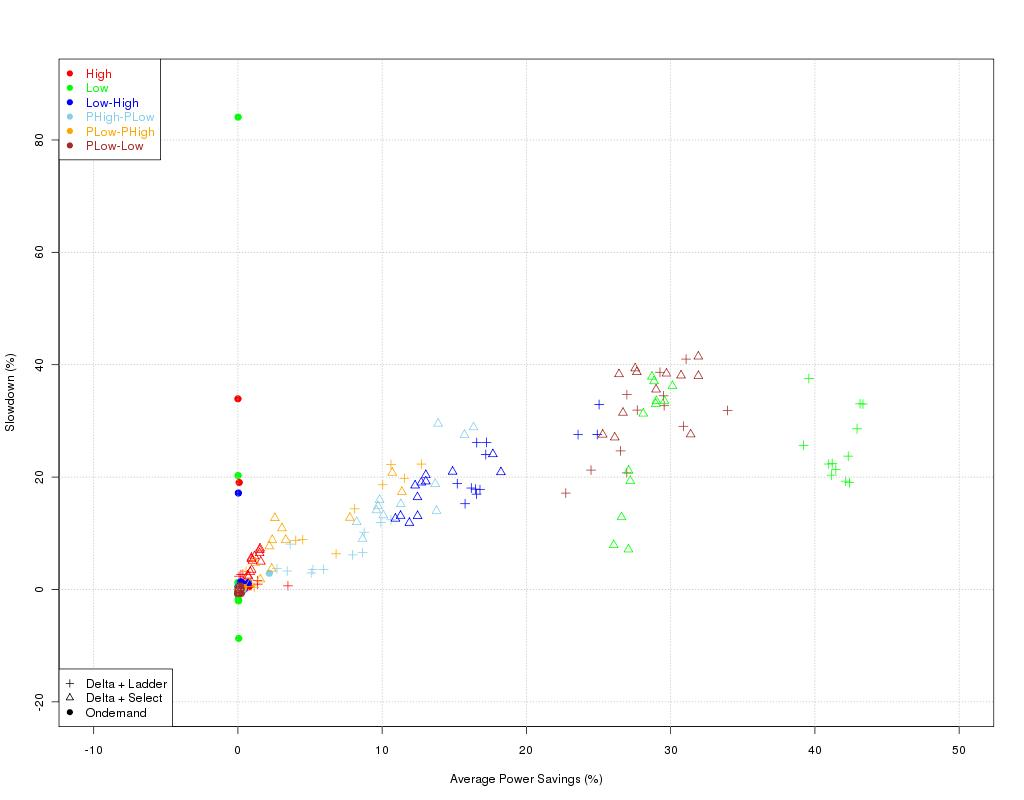
\includegraphics[height=3.0in]{figures/pwr_vs_slowdown_delta_4.jpg}%}
    \caption{Scatter plots showing variation of slowdown with power savings for ondemand, $\Delta=4$ (Select and Ladder)}
    \label{fig:pwr_vs_slowdown}
  \end{center}
\end{figure}

EPI (Energy consumption per instruction) is another important metric which ties in bother throughput and power
consumption with lower values indicating better energy efficiency. EPI is plotted 
against power savings for each experiment to arrive at Figure~\ref{fig:pwr_vs_jpbi}. As the ondemand governor
does not manage power at execution time, it is observed that not only does it not provide any power savings, 
it ends up utilizing energy inefficiently. Note that the value of EPI for the ondemand governor can be as high
as 170 nW/instruction while both the ladder and select systems exhibit a max EPI of 140 nW/instruction. 
Figure~\ref{fig:pwr_vs_jpbi} also displays the linear relationship between EPI and power savings introduced
by both the select and ladder systems.

\begin{figure}[h!]
  \begin{center}
    %\resizebox{\columnwidth}{!}{
    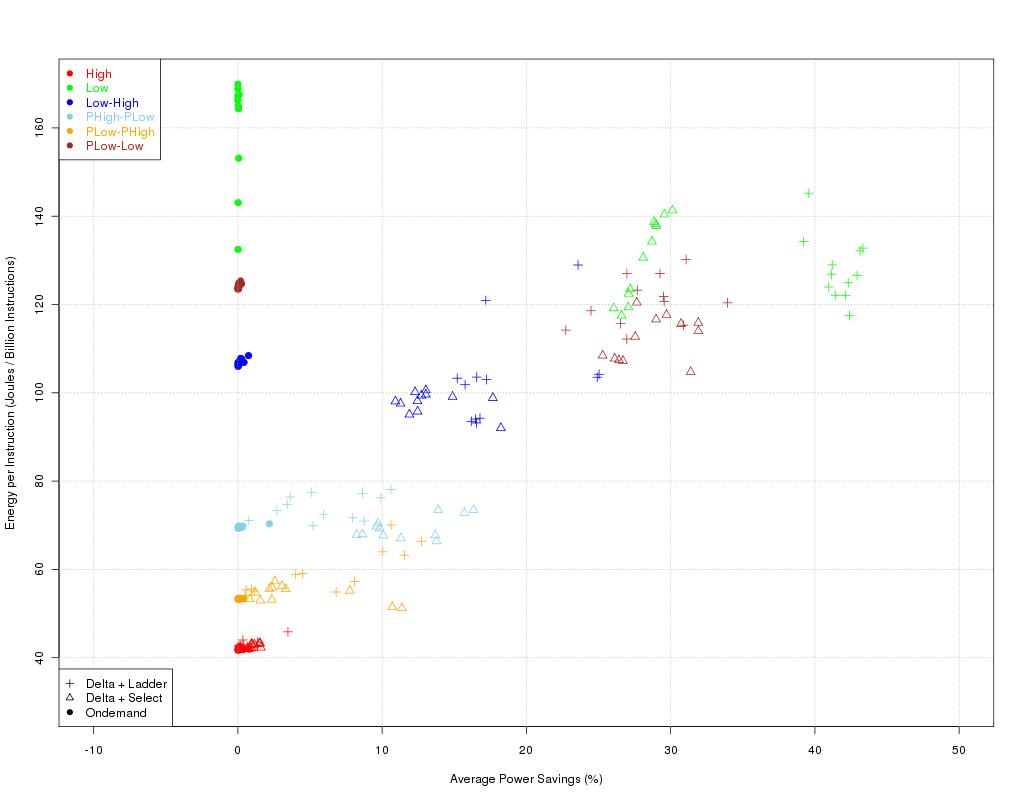
\includegraphics[height=3.0in]{figures/pwr_vs_jpbi_delta_4.jpg}%}
    \caption{Scatter plots showing variation of EPI with power savings for ondemand, $\Delta=4$ (Select and Ladder)}
    \label{fig:pwr_vs_jpbi}
  \end{center}
\end{figure}


An interesting graph Figure~\ref{fig:jpbi_vs_slowdown} is arrived at when the scatter plots concentrate on
EPI and slowdown. As we have concluded with figures \ref{fig:pwr_vs_slowdown} and \ref{fig:pwr_vs_jpbi},
the ondemand governor essentially executes all workloads at the highest clock speed (Indicated by 0 slowdown 
and power savings). This allows \ref{fig:jpbi_vs_slowdown} to be viewed to discern if the delta system
does provide a better means to execute workloads in a more energy efficient manner. This is observable
where all the points for each workload pertaining to the delta + select and delta + ladder systems lie to the left of their
respective points for the points pertaining to the ondemand optimization. A conclusion based on 
Figure~\ref{fig:jpbi_vs_slowdown} can be made to assert the fact that delta mutation system is more 
energy efficient than the ondemand system and equal at worst.

% NEEDS TO BE RE-GENERATED.
\begin{figure}[h!]
  \begin{center}
    %\resizebox{\columnwidth}{!}{
    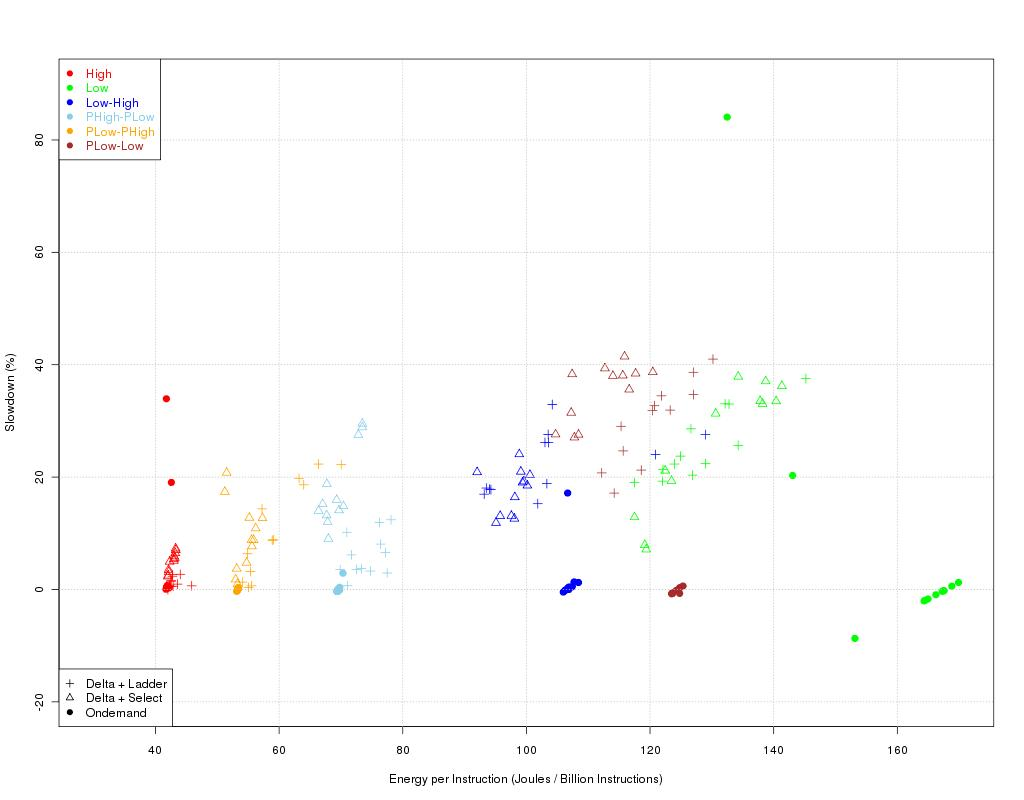
\includegraphics[height=3.0in]{figures/jpbi_vs_slowdown_delta_4.jpg}%}
    \caption{Scatter plots showing variation of slowdown with EPI for ondemand, $\Delta=4$ (Select and Ladder)}
    \label{fig:jpbi_vs_slowdown}
  \end{center}
\end{figure}

%%%%%%%%%%%%%%%%%%%%%%%%%%%%%%%%%%%%%%%%%%%%%%%%%%%%%%%%%%%%%%%%%%%%%%%%%%%%%%%
\section{Power savings and slowdown}~\label{sec:pow_slow}
%%%%%%%%%%%%%%%%%%%%%%%%%%%%%%%%%%%%%%%%%%%%%%%%%%%%%%%%%%%%%%%%%%%%%%%%%%%%%%%

The power optimizing system described in Chapters~\ref{chap:pds} and \ref{chap:delta} are shown
to introduce slowdown and hence deteriorate performance. This section describes experiments 
performed to estimate the relationship between slowdown and power savings. Each of the six
workloads were executed on both the ladder and the select systems with varying parameters
(delta from 3 to 16, and mutation interval from 125ms to 1000ms). The results of the experiments
were plotted with power savings as a function of slowdown in order to characterize potential 
power savings for an arbitrary observed slowdown. The data was estimated as a linear function
using a linear regression model shown in Figure~\ref{fig:regression}. The scatter plots along
with the regression model for the ladder and select scheduling system is shown in Figures~\ref{fig:slowdown_power_ladder}
and \ref{fig:slowdown_power_select} displaying the accuracy of the regression model. 

\begin{figure}[h!]
   \begin{equation*}
      \text{Power Savings (Ladder)} = (1.003 \times \text{Slowdown}) + 0.935
    \end{equation*}
    \begin{equation*}
     \text{Power Savings (Select)}  = (0.783 \times \text{Slowdown}) + 0.416
  \end{equation*}
  \caption{regression models for the ladder and select scheduling systems}
  \label{fig:regression}
\end{figure}

\begin{figure}[h!]
  \begin{center}
    %\resizebox{\columnwidth}{!}{
    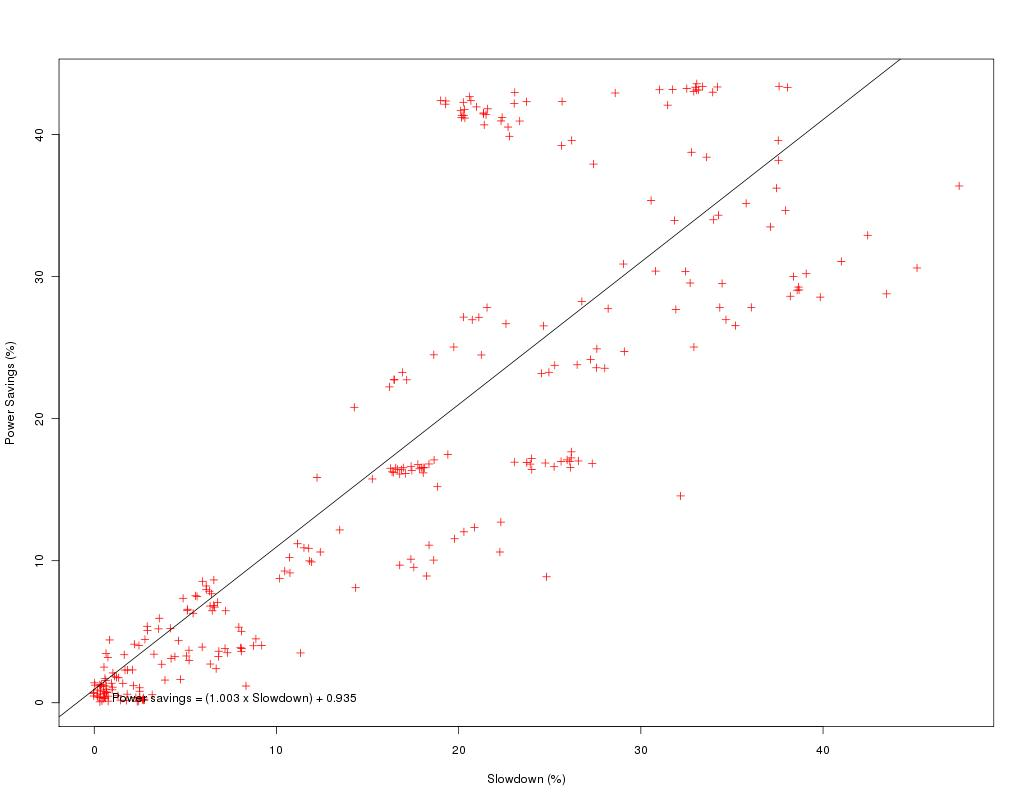
\includegraphics[height=3.0in]{figures/slowdown_power_ladder.jpg}%}
    \caption{Trends over workload variation}
    \label{fig:slowdown_power_ladder}
  \end{center}
\end{figure}

\begin{figure}[h!]
  \begin{center}
    %\resizebox{\columnwidth}{!}{
    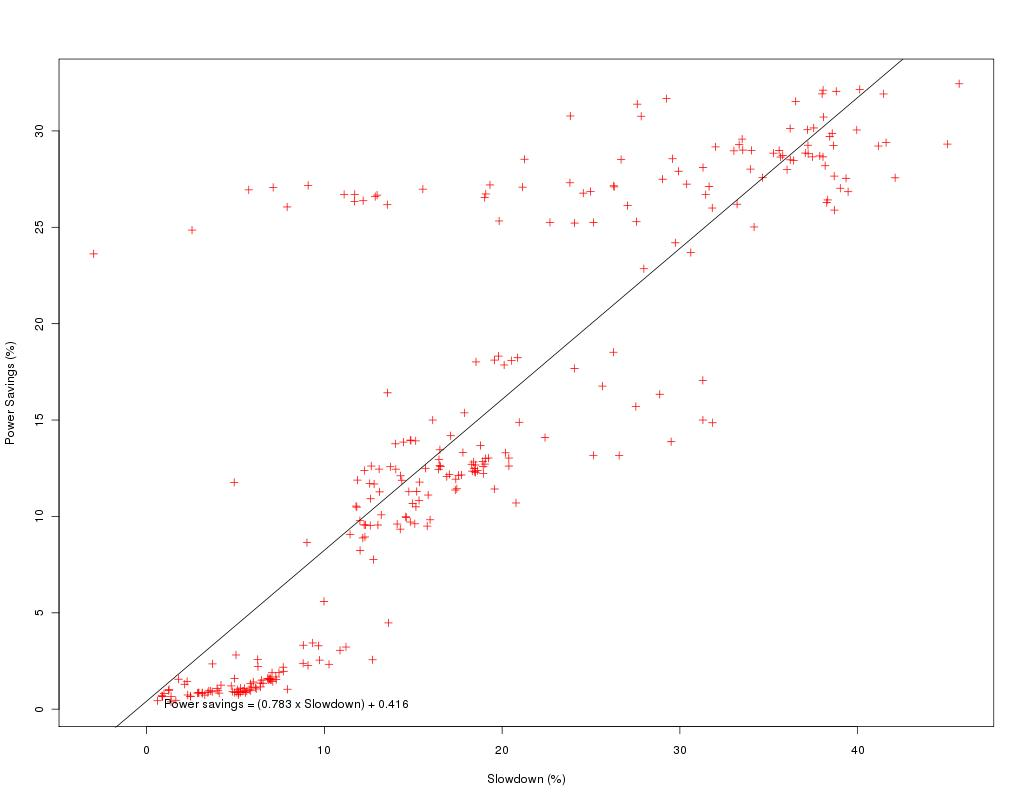
\includegraphics[height=3.0in]{figures/slowdown_power_select.jpg}%}
    \caption{Trends over workload variation}
    \label{fig:slowdown_power_select}
  \end{center}
\end{figure}

It can be observed that the ladder scheduling system along with the delta constrained mutator 
provide equal amount of power savings for every percentage of performance lost while a lower 
value of around 0.8\% of power savings can be expected from the select scheduling system for
the same amount of performance lost. Note that these are descriptive models to provide an
workload agnostic view of the power management system and are not real behavior as larger
power savings were achieved with minimum performance loss as demonstrated in earlier sections. 
%%%%%%%%%%%%%%%%%%%%%%%%%%%%%%%%%%%%%%%%%%%%%%%%%%%%%%%%%%%%%%%%%%%%%%%%%%%%%%%
\chapter{Future work}~\label{chap:future}
%%%%%%%%%%%%%%%%%%%%%%%%%%%%%%%%%%%%%%%%%%%%%%%%%%%%%%%%%%%%%%%%%%%%%%%%%%%%%%%
%%X1 Future Work

The scheduling methodology can integrate the work presented in \cite{PredictionModel}
for higher accuracy in predicting the performance state required by a particular task. 
The fact that there exists a correlation between
IPC and speedup can be utilized to produce a more robust system. The first
steps would be to provide strong support within the Linux kernel for asymmetric
multiprocessors which will enable further study into the aspect of performance
directed scheduling. 

%%%%%%%%%%%%%%%%%%%%%%%%%%%%%%%%%%%%%%%%%%%%%%%%%%%%%%%%%%%%%%%%%%%%%%%%%%%%%%%
\chapter{Summary and Conclusion}~\label{chap:conclusion}
%%%%%%%%%%%%%%%%%%%%%%%%%%%%%%%%%%%%%%%%%%%%%%%%%%%%%%%%%%%%%%%%%%%%%%%%%%%%%%%
%%X1 Conclusion

This thesis presented an approach of scheduling tasks on an asymmetric chip-multiprocessor
with respect to performance requirements and performing a constrained system wide
dynamic voltage and frequency transitions in reaction to the demands of the
performance characteristic of the executing workloads. A novel methodology was
presented in controlling the magnitude of these transitions to improve stability
and longevity of the multi-processor system. The methodology was shown to possess 
characteristics to minimize slowdown of workloads while improving the power savings achieved. 

Workloads were shown to possess characteristics to possibly make it immune to clock 
speed improvements thus enhancing the motivation of a performance determined power
management system to conserve power during system active state. Experiments with various 
static layouts were executed to characterize and showcase 
the performance directed scheduler. It was demonstrated that a statically assigned
performance state layout of a system can prove to drastically deteriorate performance 
of the system in an environment with non-deterministic workloads sets. 
Two scheduling systems, the ladder and select, were developed to schedule tasks based on
their performance characteristic.

A system was developed to allow a performance directed scheduler to direct an asynchronously
run power optimizer to manage the performance states of each processor in an otherwise 
homogeneous multi-processor environment. The problem was shown to be NP-Hard and an 
efficient algorithm was developed in solving the Multiple-choice knapsack problem 
as a direction based iterative greedy algorithm.

Experiments were conducted to measure slowdown and power savings along the system's entire
parameter space to determine the most favorable constraint on the magnitude of the 
allowed DVFS transitions. This was utilized to compare the power management system
with a popular load based power optimizer, the \textit{ondemand} governor.
The combination of the performance directed scheduler and the delta constrained mutator
was shown to achieve higher power efficiency and better power savings with a marginal 
slowdown.


%%%%%%%%%%%%%%%%%%%%%%%%%%%%%%%%%%%%%%%%%%%%%%%%%%%%%%%%%%%%%%%%%%%
%%%%%%%%%%%%%%%%%%%%%%%  Bibliography %%%%%%%%%%%%%%%%%%%%%%%%%%%%%
%%%%%%%%%%%%%%%%%%%%%%%%%%%%%%%%%%%%%%%%%%%%%%%%%%%%%%%%%%%%%%%%%%%

\bibliographystyle{IEEEtran}	% or "siam", or "alpha", or "abbrv"
				% see other styles (.bst files) in
				% $TEXHOME/texmf/bibtex/bst

%\nocite{*}		% list all refs in database, cited or not.

\bibliography{thesis}		% bib database file refs.bib

%%%%%%%%%%%%%%%%%%%%%%%%%%%%%%%%%%%%%%%%%%%%%%%%%%%%%%%%%%%%%%%%%%%
%%%%%%%%%%%%%%%%%%%%%%%%  Appendices %%%%%%%%%%%%%%%%%%%%%%%%%%%%%%
%%%%%%%%%%%%%%%%%%%%%%%%%%%%%%%%%%%%%%%%%%%%%%%%%%%%%%%%%%%%%%%%%%%

\appendix	% don't forget this line if you have appendices!
\input appA.tex			% file with Appendix A contents
\input appB.tex			% file with Appendix B contents
\input appC.tex			% file with Appendix C contents
\input appS.tex			% file with Appendix D contents

%%%%%%%%%%%%%%%%%%%%%%%%%%%%%%%%%%%%%%%%%%%%%%%%%%%%%%%%%%%%%%%%%%%
%%%%%%%%%%%%%%%%%%%%%%%%   THE END   %%%%%%%%%%%%%%%%%%%%%%%%%%%%%%
%%%%%%%%%%%%%%%%%%%%%%%%%%%%%%%%%%%%%%%%%%%%%%%%%%%%%%%%%%%%%%%%%%%

\end{document}
